%; whizzy paragraph
%; whizzy-paragraph "^\\\\dancersection"
% -initex iniptex -latex platex -format platex -bibtex jbibtex -fmt fmt
% 以上 whizzytex を使用する場合の設定。

%     Tokyo Debian Meeting resources
%     Kansai Debian Meeting resources
%     Copyright (C) 2012 Junichi Uekawa
%     Copyright (C) 2012 Nobuhiro Iwamatsu
%     Copyright (C) 2012 Koichi Akabe

%     This program is free software; you can redistribute it and/or modify
%     it under the terms of the GNU General Public License as published by
%     the Free Software Foundation; either version 2 of the License, or
%     (at your option) any later version.

%     This program is distributed in the hope that it will be useful,
%     but WITHOUT ANY WARRANTY; without even the implied warranty of
%     MERCHANTABILITY or FITNESS FOR A PARTICULAR PURPOSE.  See the
%     GNU General Public License for more details.

%     You should have received a copy of the GNU General Public License
%     along with this program; if not, write to the Free Software
%     Foundation, Inc., 51 Franklin St, Fifth Floor, Boston, MA  02110-1301 USA

%  preview (shell-command (concat "evince " (replace-regexp-in-string "tex$" "pdf"(buffer-file-name)) "&"))
% 画像ファイルを処理するためにはebbを利用してboundingboxを作成。
%(shell-command "cd image2012-natsu; ebb *.png")

% progress memo:
% 2013/12-2014/05がマージ対象、関西は2013/12-2014/05(仮)
% イベント等でない場合は理由を書くこと。
% 必要な変更点は FIXME で記録しています。

%%ここからヘッダ開始。

\documentclass[mingoth,a4paper]{jsarticle}
\usepackage{monthlyreport}
\usepackage{supertabular}
\usepackage{subfigure}
\renewcommand*\thesubfigure{}

\usepackage{comment}

% ルビ for 201312tokyo
\def\ruby#1#2{%
\leavevmode
\setbox0=\hbox{#1}\setbox1=\hbox{\tiny#2}%
\ifdim\wd0>\wd1 \dimen0=\wd0 \else \dimen0=\wd1 \fi
\hbox{\kanjiskip=\fill
\vbox{\hbox to \dimen0{\tiny \hfil#2\hfil}%
\nointerlineskip
\hbox to \dimen0{\hfil#1\hfil}}}}

% section の代わりの環境 -- 改訂する。
\renewcommand{\dancersection}[2]{%
\newpage
あんどきゅめんてっど でびあん 2014年夏号
%
% top line
\vspace{0.1mm}\\
{\color{dancerdarkblue}\rule{\hsize}{2mm}}

%
% middle text
%
\begin{minipage}[t]{0.6\hsize}
\color{dancerdarkblue}
\vspace{1cm}
\section{#1}
\hfill{}#2\\
\end{minipage}
\begin{minipage}[t]{0.4\hsize}
\vspace{-2cm}
\hfill{}\includegraphics[height=8cm]{image200502/openlogo-nd.eps}\\
\vspace{-5cm}
\end{minipage}
%
% bottom line
{\color{dancerlightblue}\rule{0.66\hsize}{2mm}}
%
\vspace{2cm}
}
% end of dancersection.

\begin{document}

\begin{titlepage}
\thispagestyle{empty}

\hspace*{-2.5cm}

\includegraphics{image2012-natsu/gudeb.eps}\\
\vspace*{0.1cm}

\vspace*{2cm}
\rotatebox{10}{\fontsize{32}{32} {\gt 東京エリア/関西Debian勉強会}}

\vspace*{-1.5cm}
\hspace*{11cm}\includegraphics[height=6cm]{image200502/openlogo-nd.eps}\\
\vspace*{0.1cm}
\hfill あんどきゅめんてっど でびあん 2014年夏号 2014年8月12日 初版発行
\end{titlepage}

\newpage
\thispagestyle{empty}\mbox{}
\newpage

\setcounter{page}{1}
\begin{minipage}[]{0.2\hsize}
 \definecolor{titleback}{gray}{0.9}
 \colorbox{dancerlightblue}{\rotatebox{90}{\fontsize{80}{80}
{\gt \color{dancerdarkblue}デビアン勉強会} }}
\end{minipage}
\begin{minipage}[]{0.8\hsize}
\hrule
\vspace{1mm}
\hrule
\setcounter{tocdepth}{1}
{\small
\begin{multicols}{2}
  \tableofcontents
\end{multicols}
} %FIXME: does not fit in one column! しかし二段にするとあまり美しくない? 真ん中のあたりで章番号とページ数の番号が近くにあるのがバランス良くない気がする
\vspace{1mm}
\hrule
\vspace{3cm}

\end{minipage}

% FIXME: 本文を追加すること。
%-------------------------------------------------------------------------------
\dancersection{Introduction}{上川 純一, 山下 尊也}
%-------------------------------------------------------------------------------

\subsection{東京エリアDebian勉強会}

 Debian勉強会へようこそ。これからDebianの世界にあしを踏み入れると
 いう方も、すでにどっぷりとつかっているという方も、月に一回Debianについ
 て語りませんか?

 Debian勉強会の目的は下記です。

\begin{itemize}
 \item \underline{Debian Developer} (開発者)の育成。
 \item 日本語での「\underline{開発に関する情報}」を整理してまとめ、アップデートする。
 \item \underline{場}の提供。
 \begin{itemize}
  \item 普段ばらばらな場所にいる人々が face-to-face で出会える場を提供
	する。
  \item Debian のためになることを語る場を提供する。
  \item Debianについて語る場を提供する。
 \end{itemize}
\end{itemize}

 Debianの勉強会ということで究極的には参加者全員がDebian Packageをがりがり
 と作るスーパーハッカーになった姿を妄想しています。情報の共有・活用を通し
 て Debianの今後の能動的な展開への土台として、「場」としての空間を提供す
 るのが目的です。

\subsection{関西 Debian 勉強会}

 関西 Debian 勉強会はDebian GNU/Linux のさまざ
 まなトピック(新しいパッケージ、Debian 特有の機能の仕組、Debian 界隈で起
 こった出来事、などなど)について話し合う会です。

 目的として次の三つを考えています。
 \begin{itemize}
  \item メーリングリストや掲示板ではなく、直接顔を合わせる事での情報交換の促進
  \item 定期的に集まれる場所
  \item 資料の作成
 \end{itemize}

 それでは、楽しい一時をお楽しみ下さい。

%-------------------------------------------------------------------------------
% end of header
%-------------------------------------------------------------------------------

\clearpage
\newpage
%201312tokyo
%-------------------------------------------------------------------------------
\dancersection{Debian GNU/Hurd 2013}{野島 貴英}
%-------------------------------------------------------------------------------
\index{debian-gnu-hurd}

\subsection{はじめに}

 2013年5月21日に、Debian GNU/Hurd 2013がリリースされました\cite{news-release-hurd}。
 今回は、このDebian GNU/Hurd 2013を
\begin{itemize}
\item インストールしてみたり、
\item 試したり
\item 調べたり
\end{itemize} 
した事を書いてみます。

\subsection{インストールしてみる}

 Debian GNU/Hurd 2013のインストールCDイメージは、Hurdベースのネットワークインストール可能なイメージになっています。ここでは、実際にLinuxのKVMを使い、Debian GNU/Hurd 2013をインストールして動かしてみます。

 なお、Debian GNU/Hurd 2013は、i386アーキテクチャが対象ですが、AMD64(64bit)環境のKVM上でそのまま何ら問題なく動作します。

\begin{description} 
\item [Step 1.] debian sidを用意し、過去の東京エリアDebian勉強会のKDE開発環境の資料\cite{kde-devel-debian}を参考に、br0デバイスをセットアップしておき、インターネットへアクセスできる環境を用意しておきます。
\item [Step 2.] Debian GNU/Hurd 2013のNETINST CDイメージを入手します。
\begin{commandline}
$ wget http://ftp.debian-ports.org/debian-cd/hurd-i386/current/debian-hurd-2013-i386-NETINST-1.iso
\end{commandline}
%$
\item [Step 3.] KVMを使い、インストールします。コツとして、ディスクI/OはIDE、ネットワークデバイスはe1000を利用するとよいです。
\begin{commandline}
$ sudo aptitude install libvirt-bin virtinst
$ sudo qemu-img create -f raw /var/lib/libvirt/images/debian-hurd0 7G
$ sudo virt-install --connect=qemu:///system -n debian-hurd0 --ram 512 \
  --cdrom /home/yours/debian-hurd-2013-i386-NETINST-1.iso \
  --disk /var/lib/libvirt/images/debian-hurd0,bus=ide,size=7,format=raw,cache=writeback \
  --bridge=br0,model=e1000 --vnc --hvm --accelerate
\end{commandline}
%$
また、インストーラで訊かれる質問は表\ref{tab:hurd-install-qa}のようにしています。
\begin{table}[ht]
\begin{center}
\begin{tabular}{|l|l|l|p{5cm}|}
\hline 
項番&項目名&値 &備考\\ \hline \hline
1 & country & other→Asia→Japan & \\ \hline
2 & Configure locales & United States en\_US.UTF-8 & \\ \hline
3 & Configure the keyboard & おつかいのキーボードにて & 106キーは無い\\ \hline
4 & NetworkConfigure Manually & 192.168.0.2等 & お使いの環境にて \\ \hline
5 & Partition disk & "Guided - use entire disk"	& 簡易的にこちらを選択。\\ \hline
6 & mirror country & Japan指定の、ftp.jp.debian.orgを選択 & \\ \hline
\end{tabular}
\end{center}
\caption{インストーラでの質問への回答例}
\label{tab:hurd-install-qa}
\end{table}

なお、インストール中''Select and install software''メニューで、
``Debian desktop environment''を指定していると、インストーラが途中で異常終了してしまいます。その時は諦めて、一旦''Debian desktop environment''をインストール候補から外してみて、Step 3.からやり直しとなります。\footnote{自分がやった時は、xserver-xorg-video-allのパッケージ依存関係が満たせなかった様です。今は治っているかもしれません。}
\item [Step 4.] インストールが完了すると、勝手にブートしてvirt-viewerにてGNU/Hurdが立ち上がり、''login:''プロンプトが出ますので、ログインすると使えます。
\end{description}

\subsection{使うにあたってちょっと知ると良いこと}

 基本的にはUNIX系システムの使い勝手です。Debian GNU/Linux使える方なら、非常にとっつき易い感じです。もちろんですが、Debianなので、dpkg/aptはそのまま使えます。

 ただ、hurdを使うにあたって、いくつかLinuxとは違う点があるので、知ると便利な件をいくつか以下に記載します。

\begin{enumerate}
\item システム停止 \\
Linuxシステムですと、/sbin/shutdown -h now とか、CTL+ALT+DELのキーアクションとかが一般的かと思いますが、hurdの場合は sync;haltとなります。shutdownをhurdで利用すると解るのですが、initと連携できなくてshutdownコマンドが途中で失敗します。
\item ネットワーク関係の設定 \\
Linuxシステムですと、ipコマンドとか、ifconfigコマンドとかありますが、
hurdですとsettransコマンド使って、/hurd/ディレクトリ以下のネットワーク用のtranslatorというコマンド群と、特定のデバイスファイルを結びつけるという事で対応します。
\begin{commandline}
NIC設定の例:
# settrans -fgcap /servers/socket/2 /hurd/pfinet -i eth0 \
     -a 192.168.0.5 -m 255.255.255.0 -g 192.168.0.1
\end{commandline}
 また、hurdの場合、translatorへfsysoptsコマンドで指示を出すことにより、translatorが対応していれば設定変更もできます。
\begin{commandline}
NICの設定がどうなっているか?
# fsysopts /servers/socket/2
/hurd/pfinet --interface=/dev/eth0 --address=10.3.0.1 --netmask=255.255.0.0 --gateway=10.3.0.128
(ps -auxww | fgrep pfinetとかしても可)
NIC設定変更の例:
# fsysopts /server/socket/2 -a 10.3.0.2 -m 255.255.0.0 -g 10.3.0.128 
\end{commandline}
\item ファイルシステムのマウント\\
Linuxだとmountコマンドですが、hurdの場合ですと、
\begin{commandline}
物理デバイスをマウント
# settrans /mnt /hurd/ext2fs /dev/hd0s5
CDイメージをマウント
# settrans /mount/point /hurd/iso9660fs CD_image.iso
NFSをマウント
# settrans -cgap /mount/point /hurd/nfs 192.168.1.1:/home
\end{commandline}
という形で、ファイルシステム用のtranslatorをsettransコマンドでマウントポイントに結びつけてしまうという手を使います。
\end{enumerate}

 その他については、Debian GNU/Hurd Configuration(\url{http://www.debian.org/ports/hurd/hurd-install})を見ると良いです。

\subsection{Xを動かしてみる}

 ログインしてそのままCUIで利用という\ruby{漢}{おとこ}な使い方も確かにできますが、Xぐらいは動かしたい場合もあるわけです。試しに動かしてみます。

\begin{commandline}
# aptitude install xserver-xorg-video-cirrus xinit fluxbox
# xinit
ここで、白いウィンドウが出るので、そのウインドウにカーソルを合わせ、
# fluxbox &
\end{commandline}

 慣れてきたら、/root/.xinitrcとかにいろいろ書くと便利です。

 なお、今回Xをrootで動かしています。本来、一般ユーザで動かせると良いのですが、
自分はまだしっかり調べきれていません。

\subsection{GNU Hurd図解}

  GNU Hurdを図解してみます。

\begin{figure}[H]
\begin{center}
 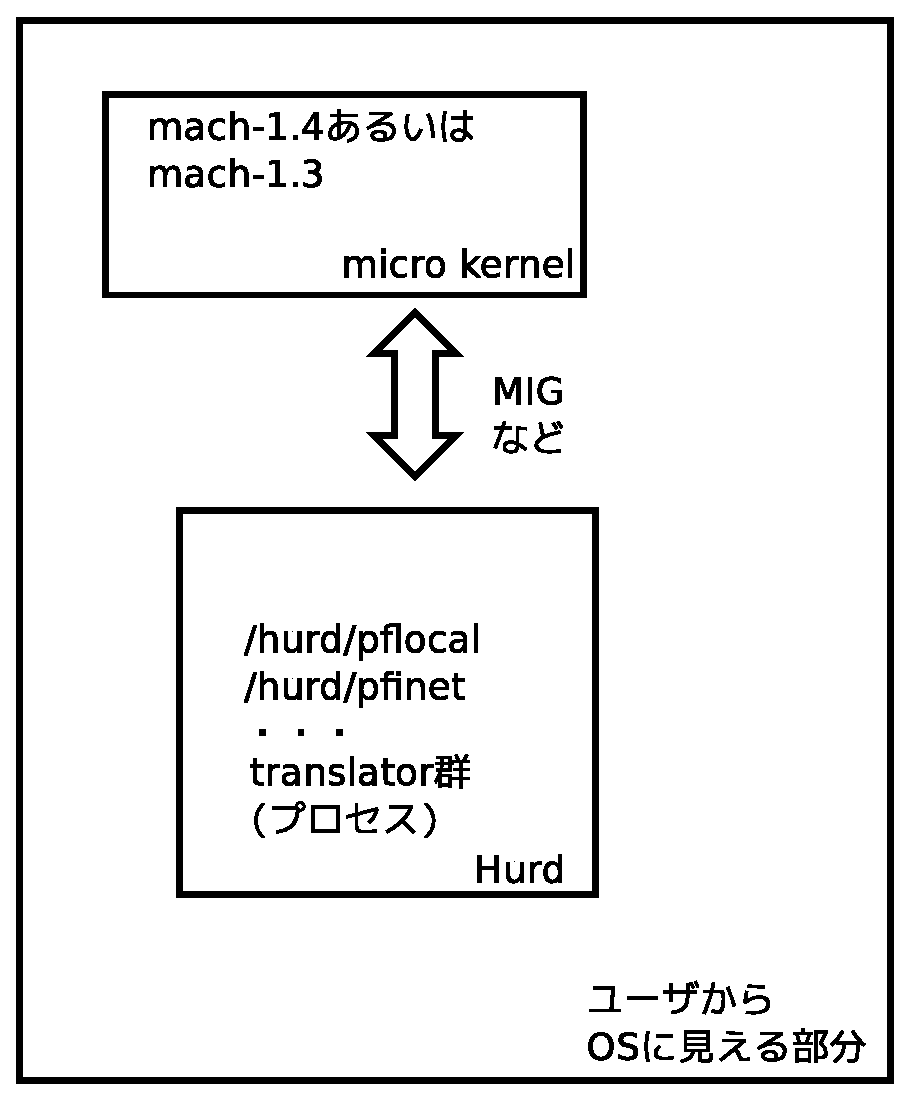
\includegraphics[scale=0.3]{image201312/gnu-hurd-schema.eps}
 \caption{OSの図解}\label{fig:gnu-hurd-schema}
\end{center}
\end{figure}

 図のとおり、

\begin{itemize}
\item カーネル本体はmach-1.3/1.4
\item ファイルシステム、ネットワークインターフェースなどは/hurd/以下にあるtranslatorと呼ばれる実行バイナリによるユーザプロセス
\item カーネル本体とtranslator群は主にMIGと呼ばれるRPCなどで通信
\end{itemize}

という構造になっています。

\subsection{終わりに}

 Debian GNU/Hurd は、まだいろいろと未開拓な部分も多いです。また、
gnu hurd本体もいろいろと他に機能が必要な状態です。

 すでにいろいろと完成されたDebian GNU/Linuxも面白いですが、
いろいろ未完成なDebian GNU/HurdもHackして遊ぶには面白いと
思います。皆様もぜひ。

\begin{thebibliography}{0}
  \bibitem{news-release-hurd}
    {\footnotesize{
       Debian.org,``Debian GNU/Hurd 2013 リリース!'',
       \url{http://www.debian.org/ports/hurd/hurd-news}
       }}
  \bibitem{kde-devel-debian}
    {\footnotesize{
       野島 貴英,「Debian開発者のKDE環境あれこれ」,第85回東京エリアDebian勉強会資料,
       \url{http://tokyodebian.alioth.debian.org/pdf/debianmeetingresume201202.pdf}
       }}
\end{thebibliography}

%201401 tokyo
%-------------------------------------------------------------------------------
\dancersection{Debian Pure Blend}{野島 貴英}
%-------------------------------------------------------------------------------
\index{debian-pure-blends}

\subsection{Debian Pure Blend}

 Debianに用意されている大量のパッケージをうまく使い、そのままのDebianのリポジトリを用いる事で、特定分野向けのシステムを容易にセットアップできるようにしたDebianの仕組み(考え方)となります。

 Debianパッケージに含まれるRecommends情報が利用されて、指定された特定用途のパッケージが導入される仕組みとなっています。

\subsection{用語}

 Debian Pure Blendを語る時に使われる用語を以下に載せておきます\cite{debian-pure-blends-wiki}。

\begin{table}[ht]
\begin{center}
\begin{tabular}{|l|l|p{9cm}|p{3cm}|l|}
\hline 
項番&呼び名&概要&備考 \\ \hline \hline
1 & Debian Pure Blend & そのままのDebianを用いて特定用途向けのDebianを実現 & DebiChem, Debian Edu等 \\ \hline
2 & Debian Blend & 一部のDebianでは未だ公式には採択されていないちょっとした変更を付け足し、残りはそのままのDebianを用いて特定用途向けのDebianを実現 & \\ \hline
3 & Debian Derivative & Debian派生物と日本語では言われる。目的は様々であり、Debianを元にした新しいディストリビューションを作るという点では共通。Debianをベースにしたかもしれないが、現在では大量の変更/新規機能を加えて作られているディストリビューション。& ubuntu, SteamOS \\ \hline
4 & web sentinel & \url{http://blends.debian.org}。PureBlendの種類と搭載されているパッケージ及び開発状況を載せているページ。 & \\ \hline
\end{tabular}
\label{tab:debian-blends-terms}
\caption{用語}
\end{center}
\end{table}

\subsection{利用できるPure Blend}

 現在Debian unstableで見つかったPure Blend用のパッケージの一覧を載せます。

\begin{table}[ht]
\begin{center}
\begin{tabular}{|l|l|l|p{5cm}|l|}
\hline 
項番&用途& PJ名前 & 概要&メタパッケージ名 \\ \hline \hline
1 & 子供用 & Debian Junior & 子供向けのDebianを作る & junior-* \\ \hline 
2 & 医療 & Debian Med  & 医療関係者向けのDebianを作る & med-* \\ \hline 
3 & 学校 & Debian Edu & 学校の情報教育向けのDebianを作る & education-*,debian-edu-* \\ \hline 
4 & 科学技術 & Debian Science & 科学技術向けのDebianを作る & science-* \\ \hline 
5 & マルチメディア & Debian Multimedia & マルチメディア作成関係者向けのDebianを作る & multimedia-* \\ \hline 
6 & 地理情報 & DebianGIS & 地理関係者向けのDebianを作る & gis-* \\ \hline 
7 & 化学 & Debichem & 化学関係者向けのDebianを作る & debichem-* \\ \hline 
8 & 中国語対応の一例 & Debian EzGo & 中国語に対応したDebianの1つを作る & ezgo-* \\ \hline 
\end{tabular}
\label{tab:debian-blend-package}
\caption{Debian unstableで見つかるPure Blend}
\end{center}
\end{table}

 なお、経緯を追いかけきれていないのですが、''Existing Debian Pure Blends''に記載されている他のBlendのパッケージ\cite{debian-existing-blends}を自分は見つけることができませんでした。

\subsection{使ってみる}

 早速使ってみます。ここでは、Debian Juniorを選んでみます。

\begin{description}
\item [Step 1.] debianを用意しgnome desktopを導入しておきます。
\item [Step 2.] Debian Juniorのメタパッケージの一つである、junior-gnomeを入れてみます。
\begin{commandline}
$ sudo aptitude install junior-gnome
... junior-gnome/compris/gworldclock/mathwarが導入される...
\end{commandline}
%$
\end{description}

 gnomeのメニューを見ると、gcompris/gworldclock/mathwarが新規に増えている事が分かります。

\subsection{仕組み}

 Pure Blendのパッケージは、Recommendsとしてに導入したい特定用途向けのアプリケーションが指定されています。そのため、Pure Blendのパッケージを導入すると、Recommendsに指定されたアプリケーションがまとめて導入されます。

 試しに、先の例のjunior-gnomeの依存関係を調べてみます。

\begin{commandline}
$ apt-cache depends junior-gnome
  Depends: junior-tasks
  Depends: junior-config
  Recommends: gcompris
  Recommends: gworldclock
  Recommends: mathwar
\end{commandline}
%$
 
 Recommendsとして、gcompris/gworldclock/mathwarが指定されている事がわかります。

\subsection{Pure Blend用のパッケージを作ってみる}

 Pure Blend用のパッケージを試しに作ってみます。blends-devパッケージを
導入することで、taskファイルからPure Blend用のパッケージを簡単に作る事ができます。

 ここでは、例として、ゲームのジャンルでvisual novelを選び、これらのパッケージ
を導入するようなパッケージを作成してみます。

\begin{table}[ht]
\begin{center}
\begin{tabular}{|l|l|p{5cm}|}
\hline 
項目& 内容 & 説明\\ \hline \hline
PJ名 & Debian-visualnovel & visualnovel用途向け \\ \hline 
パッケージ名 & visualnovel-* & visualnovelメタパッケージ \\ \hline 
tasksel用パッケージ & visualnovel-task & tasksel用定義ファイル \\ \hline 
\hline 
\end{tabular}
\label{tab:debian-visualnovel}
\caption{今回のPure Blendの定義}
\end{center}
\end{table}


\begin{description}
\item [Step 1.] blends-devパッケージを導入します。
\begin{commandline}
$ sudo aptitude install blend-dev
\end{commandline}
%$
\item [Step 2.] 作業ディレクトリを作り、必要なファイルをblends-devパッケージに梱包されているテンプレートをコピーして用意します。
\begin{commandline}
$ mkdir debian-visualnovel-1.0
$ cd debian-visualnovel-1.0
$ cp -a /usr/share/doc/blends-dev/examples/config .
$ cp -a /usr/share/doc/blends-dev/examples/debian .
$ cp -a /usr/share/doc/blends-dev/examples/tasks .
$ cp /usr/share/doc/blends-dev/examples/Makefile .
$ cp /usr/share/doc/blends-dev/examples/README .
\end{commandline}
%$
\item [Step 3.] コピーした各ファイルに含まれる''\_BLEND\_''の文字列を''visualnovel''に全部置き換えます。
\begin{commandline}
$ find . -type f | xargs -n 1 sed -i 's/_BLEND_/visualnovel/g'
\end{commandline}
%$
\item [Step 4.] debian/control.stubを編集します。ここで、Packageの定義として、visualnovel-tasksを必ず追加指定しておきます。また、debian/changelogも書いておきます。
\begin{commandline}
$ vi debian/control.stub
----debian/control.stubここから-------
Source: debian-visualnovel
Section: misc
Priority: extra
Maintainer: Your Name <Your mail>
Build-Depends-Indep: debhelper (>= 9),
                     blends-dev (>= 0.6.16.4)
Standards-Version: 3.9.4

Package: visualnovel-tasks
Architecture: all
Depends: tasksel
Description: Debian visualnovel for tasksel
 This package provides Debian visualnovel tasks in tasksel. 

----debian/control.stubここまで-------
$ vi debian/changelog
----debian/changelogここから------
debian-visualnovel (1.0) unstable; urgency=low

  * initial release

 -- Your Name <your@e-mail>  Mon, 13 Jan 2014 23:56:00 +0900

----debian/changelogここまで------
\end{commandline}
\item [Step 5.] tasks/task1をtasks/gameに変更し、どのパッケージを導入するか等をDepends:行に指定します。visual novelですので、onscripterと、renpy-thequestionを入れてみます。
\begin{commandline}
$ mv task/task1 task/game
$ vi task/game
--------task/gameここから----------
Task: game
Description: Debian-visual novel games_
 This metapackage will install Debian packages for use in 
 game of Debian-visualnovel

Depends: onscripter, renpy-thequestion

--------task/gameここまで----------
\end{commandline}
\item [Step 6.] パッケージを作るために必要なファイルを自動生成します。
\begin{commandline}
$ make -f debian/rules gen-orig-source
\end{commandline}
%$
\item [Step 7.] パッケージをビルドします。
\begin{commandline}
$ debuild
...visualnovel-game/visualnovel-taskパッケージが出来上がる...
\end{commandline}
%$
\end{description}

 無事visualnovel-*パッケージができました。

\subsection{おわりに}

 今回は、Debian Pure Blendの導入から作成まで説明してみました。豊富なパッケージを持つDebianならではの考え方と思います。これを機に、皆さんも何かDebian Pure Blendを作ってみませんか?

\begin{thebibliography}{0}
  \bibitem{debian-pure-blends-wiki}
    {\footnotesize{
       Debian wiki,``DebianPureBlends'',
       \url{https://wiki.debian.org/DebianPureBlends}
       }}
  \bibitem{debian-existing-blends}
    {\footnotesize{
       blends.debian.org,''Existing Debian Pure Blends'',
      \url{http://blends.debian.org/blends/ch04.html}
    }}


\end{thebibliography}

%201405 tokyo
%-------------------------------------------------------------------------------
\dancersection{debianでdocker.io}{野島 貴英}
%-------------------------------------------------------------------------------
\index{docker.io}

\subsection{はじめに}

 去年あたりから、linuxのコンテナ環境であるdocker\cite{docker-orig}が注目されているようです。

 dockerは使うとわかるのですが、単にlinux上にコンテナ環境を作成するという機能の他に、aufsを利用してベースのOSのシステムに迅速に変更差分を適用するという動作により、非常に素早くカスタム化されたコンテナ環境の作成・変更・管理が出来ます。

 また、変更した内容をdockerリポジトリ(\url{https://index.docker.io})に登録することにより、dockerが動作する環境さえあれば、こちらのリポジトリから全く同じコンテナ環境を作成・動作させることができます。

 今回はdebianをdockerホストにしてdockerを使ってみた事について発表します。

\subsection{今回利用のdebian}

 今回発表で評価したdebianはunstable(jessie/sid)となります。

 なお、残念ながら安定版のdebian wheezyでは未だdockerはパッケージ化されていない
状況です。本誌を読まれているdebian使いの方は、ぜひこの機会にdebian unstable(jessie/sid)
にアップグレードしてパッケージからdockerをお試しください。

\subsection{docker仕組みの簡単なおさらい}

 dockerを図示すると図のようになります。

\begin{figure}[H]
\begin{center}
 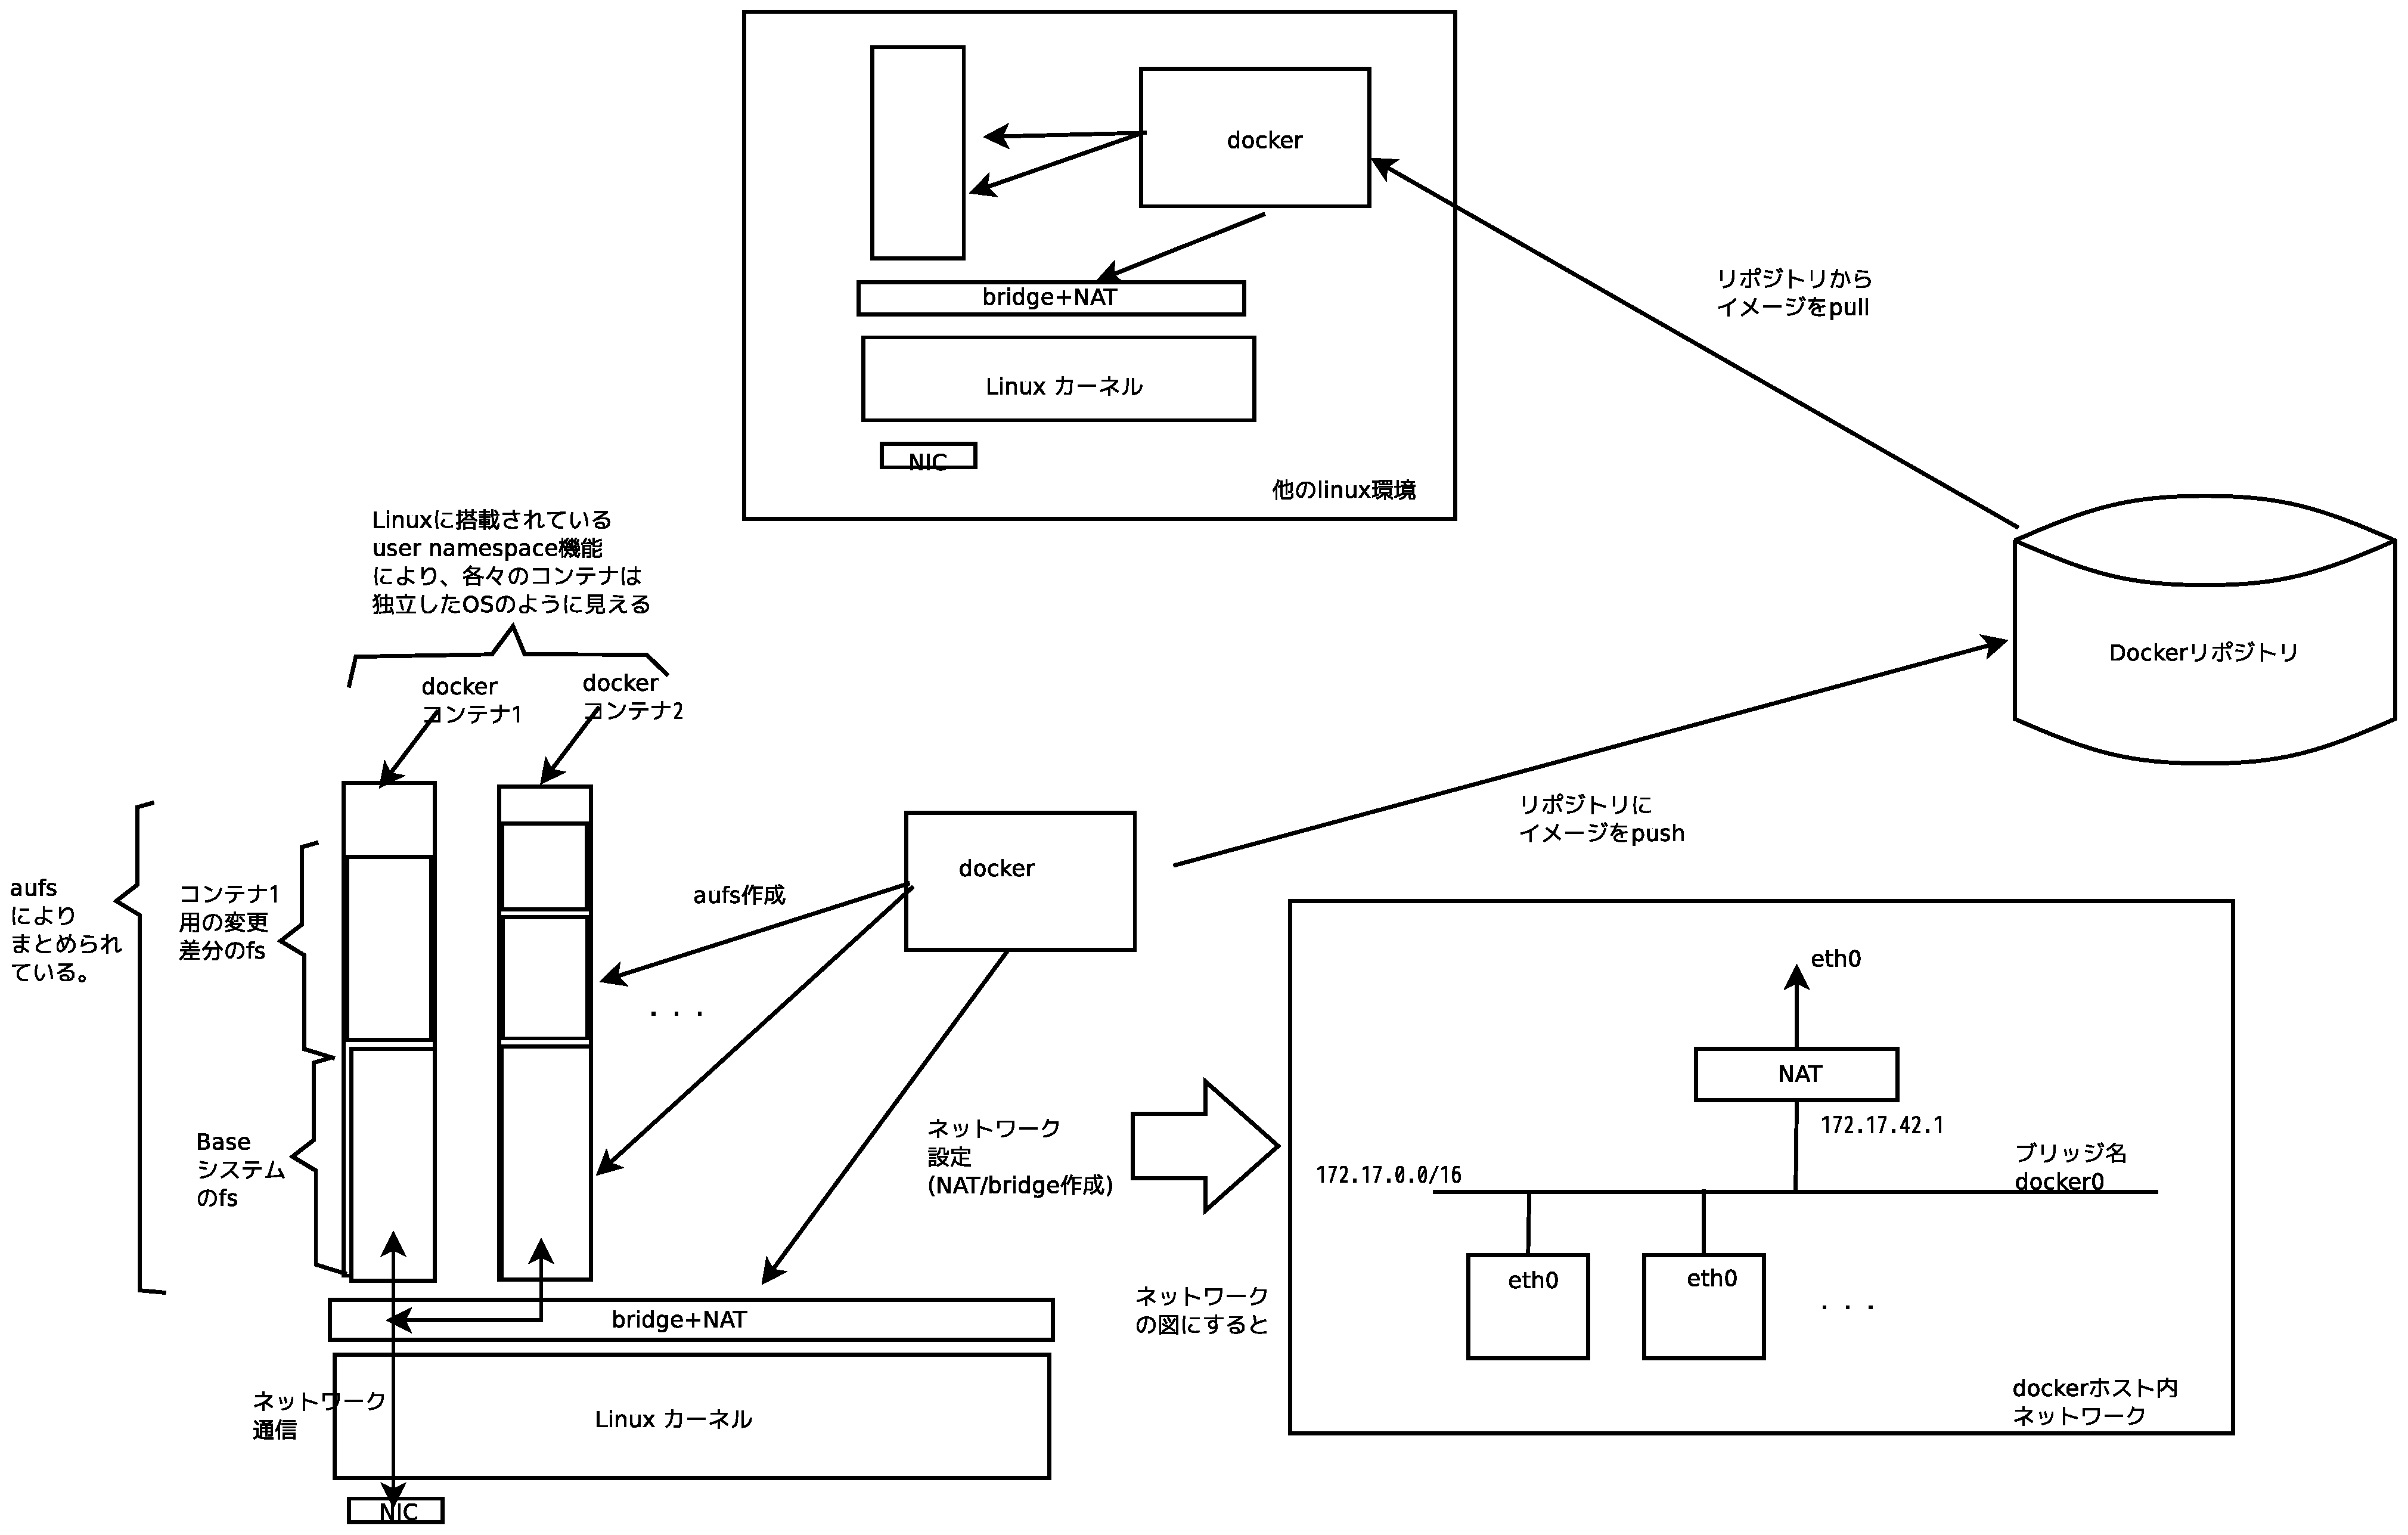
\includegraphics[width=1.0\hsize]{image201405/docker-overview.eps}
 \caption{dockerの構造}\label{fig:docker-overview}
\end{center}
\end{figure}

 dockerによるコンテナ環境の特徴としては、

\begin{itemize}
\item 非常に素早い起動、停止が可能です。
\item baseのファイルシステムに、aufsによる差分ベースのファイルシステム内容の適用を行うため、非常に簡単にコンテナの変更・破棄が可能です。
\item 構成管理をDockerリポジトリで行える。(注:一見gitのような使い方に見えますが、gitを使って作られているわけではありませんので、gitほどの高機能で柔軟な変更管理はできません)
\item Dockerリポジトリが参照でき、dockerが動く環境であれば、dockerホストのlinuxディストリビューションが異なる環境でも同じ構成内容を持つdockerコンテナを動作できます。
\end{itemize}

となります。

 dockerホストの内部のネットワークは、dockerにより、ブリッジdocker0が作成され、
dockerホストのeth0へNATされて接続されます。そのため、dockerホスト外からの
コンテナ側のサービスへのアクセスは、DNATしてdockerホスト側のポートへ引き出す
ことにより行われます。

\subsection{手元のdebian機材で試す}

 以下の手順で簡単に試すことが出来ます。
 
 \begin{description}
 \item [Step 1.] インターネットに接続できているdebian unstable環境を用意します。
 \item [Step 2.] ip forwardingができるようにしておきます。
  \begin{commandline}
$ sudo vi /etc/sysctl.d/ip-forward.conf
----ここから-----
net.ipv4.ip_forward=1
----ここまでを記載-----
$ sudo sysctl -p /etc/sysctl.d/ip-forward.conf
  \end{commandline}
%$
 \item [Step 3.] dockerを導入します。なお、debianパッケージのdockerは、docker.ioというパッケージ名であり、コマンドもdockerではなく、{\bf docker.io}という名前になります。(以降本コマンドをdocker.ioコマンドと呼びます)
  \begin{commandline}
$ sudo aptitude install docker.io
$ docker.io
Usage: docker [OPTIONS] COMMAND [arg...]
 -H=[unix:///var/run/docker.sock]: tcp://host:port to bind/connect to or unix://path/to/socket to use

A self-sufficient runtime for linux containers.

Commands:
    attach    Attach to a running container
...中略(docker.ioコマンドのhelpが出る)...
  \end{commandline}
 \item [Step 3.] グループdockerに操作者のログインIDを追加し、ログインしなおします。こうすることでdocker.ioコマンドによる操作を一般ユーザ権限で操作できるようになります。
  \begin{commandline}
$ sudo useradd YOUR-ID docker
$ exit 
login: YOUR-ID
Password: xxxxx
$ 
  \end{commandline}
 \item [Step 4.] 試しにコンテナとしてdebian-sid(jessie-sid)をdockerで動かしてみます。
  \begin{commandline}
$ docker.io run -t -i -h debian-sid1 debian:sid
Unable to find image 'debian:sid' locally
Pulling repository debian
1cda8535c670: Download complete 
511136ea3c5a: Download complete 
0ed2a4d77969: Download complete 
root@debian-sid:/#  <-- 起動したdockerコンテナのdebian sid。
  \end{commandline}

 \item [Step 5.] 作ったdockerコンテナの中でpsを導入し、processを見てみます。

  \begin{commandline}
root@debian-sid:/# apt-get install procps
root@debian-sid2:/# hash
hits	command
   2	/sbin/ip
   1	/usr/bin/apt-get
root@debian-sid2:/# ps -auxww
USER       PID %CPU %MEM    VSZ   RSS TTY      STAT START   TIME COMMAND
root         1  0.0  0.0  18016  1932 ?        Ss   22:17   0:00 /bin/bash
root       118  0.0  0.0  17488  1136 ?        R+   22:26   0:00 ps -auxww
root@debian-sid2:/# 
  \end{commandline}
 見るとわかるとおり、initの代わりに/bin/bashがPID=1で動作している状態です。
 
 \item [Step 6.] Ctrl+p Ctrl+qを連続で打ち込むと、dockerコンテナのshellから抜けます。なお、
exitを実行すると、PID=1の/bin/bashが終了するため、shutdownを実行したことと等価となり、
コンテナが終了します。
  \begin{commandline}
root@debian-sid2:/# ...ここで Ctrl+p Ctrl+qする...
$ <- dockerホストのプロンプトが帰ってくる
$ docker.io ps 
CONTAINER ID        IMAGE               COMMAND             CREATED             STATUS              PORTS               NAMES
20fa6020f73b        debian:sid          /bin/bash           12 minutes ago      Up 12 minutes                           evil_euclid
(コンテナID: 20fa6020f73bが動作中であることを示す)
$ docker.io attach 20fa6020f73b (<--再びdebian-sidに接続)
<リターンキー押す>
root@debian-sid2:/# <-再びコンテナのshellプロンプト。
root@debian-sid2:/# exit
$ docker.io ps 
CONTAINER ID        IMAGE               COMMAND             CREATED             STATUS              PORTS               NAMES
$
(docker.io psをとって稼働中のコンテナを確認したが、コンテナが終了してしまっているため、動作中のコンテナIDが表示されない↑)
 \end{commandline}
 \end{description}  

\subsection{dockerのネットワークの癖について}

 dockerは、dockerホストの起動時にdockerがデーモンモードで動作しており、dockerコマンドで
指令を送ってコンテナの管理をします。ここで、dockerホストのネットワークを、デーモンモードの
dockerが起動時にセットアップしています。

 ここで、例えばdockerホストがモバイルPCであった場合、pppとかを後から起動するなどして、
ネットワークの設定がdockerデーモンがセットアップした状態と異なってしまうことがあります(特にNAT周り。)

 この場合、docker.ioでコンテナを作成しようとしても、作成途中のコンテナ側からネットワークが外部へのネットワーク通信が出来ず、
コンテナ作成が途中で停止する現象が起きることがあります。

 この場合は、pppなどの通信をつないだ状態で、再度、dockerデーモンを再起動すると、再度
ネットワークがセットアップされ、問題が解決します。

  \begin{commandline}
$ pon xxxx <-- pppを起動などしてNATがpppの定義で書き換えられてしまう。
$ docker.io run -t -i -h debian-sid1 debian:sid
Unable to find image 'debian:sid' locally
Pulling repository debian
1cda8535c670: Download complete 
...ここでハングアップしてしまう...
(Ctrl+Cで停止させる)
$ sudo systemctl restart docker.io.service 
(dockerデーモンの再起動が行われる)
$ docker.io run -t -i -h debian-sid1 debian:sid
Unable to find image 'debian:sid' locally
Pulling repository debian
1cda8535c670: Download complete 
511136ea3c5a: Download complete 
0ed2a4d77969: Download complete 
root@debian-sid:/#  <-今度はコンテナが無事起動する。
 \end{commandline}

\subsection{GCEでdocker}

 手元のdebian機でdockerを動かすだけでは物足りないかと思います。
今年はimmutable infrastructure\cite{immuta-desc}の年ですので、
早速パブリッククラウド環境でも動かしてみることにします。

 Google Compute Engine(GCE)でもdockerは動くとのことですので、試してみます。

\begin{description}
 \item [Step 1.] お手元のdebian sidでchromiumなどのブラウザを使い、googleアカウントでgoogleにログインしておきます。
 \item [Step 2.] \url{https://developers.google.com/}のgoogle デベロッパサイトから、Google Cloudにサインアップします。\\
注意:巷のblogなどでは、\url{https://developers.google.com/compute/docs/signup}が案内されていますが、評価期間は終わっているため、こちらからサインアップする必要はありません。長い英語のアンケートに英語で答えさせられるなどの苦行が待っているため、こちらはおすすめしません。
 \item [Step 3.] プロジェクトを作成するメニューが最初に現れますので、適当にプロジェクトを作成します。
  \begin{description} 
     \item [Project Name:] docker evalation
     \item [Project ID:] docker-evaluation-test-001
   \end{description}
   \item [Step 4.] billing(支払い)メニューになるので、支払いの情報を記載します。
    \item [Step 5.] 特に折り返しの電話などなく、GCEのメニューになります。
   \item [Step 6.] お手元のdebian unstable機材に、google-cloud-sdkをダウンロードします。
     \begin{commandline}
$ mkdir google-sdk;cd google-sdk
$ wget https://dl.google.com/dl/cloudsdk/release/google-cloud-sdk.tar.gz
$ tar xzf google-cloud-sdk.tar.gz
$ cd google-cloud-sdk
$ ./install.sh
 ...カレントディレクトリにインストールが開始...
$ cd ..
$ zshの場合:source google-cloud-sdk/path.zsh.inc;rehash
  bashの場合:source google-cloud-sdk/path.bash.inc;hash
        \end{commandline}
    \item [Step 7.] sdkから認証を行います。
  \begin{commandline}
$ gcloud auth login
...ここで、chromiumなどが開き、sdkがgoogleのアカウントにアクセスしてよいかの
  許可を求められるので、「承諾」を押下...
$ 
  \end{commandline}
    \item [Step 7.] GCEのinstanceを作ります。ここでは、料金の最も安いf1-microで、ネットワーク的に近いアジア地域に、debian wheezyのイメージで作ります。3秒ぐらいで完了します。
  \begin{commandline}
$ gcutil addinstance docker-test001 --project=docker-evaluation-test-001 --image=debian-7 --machine_type=f1-micro \
--zone=asia-east1-a --wait_until_running --auto_delete_boot_disk 
INFO: Resolved debian-7 to projects/debian-cloud/global/images/debian-7-wheezy-v20140415
INFO: Waiting for insert of instance docker-test001. Sleeping for 3s.
INFO: Waiting for insert of instance docker-test001. Sleeping for 3s.
INFO: Waiting for insert of instance docker-test001. Sleeping for 3s.
INFO: Waiting for insert of instance docker-test001. Sleeping for 3s.
INFO: Ensuring docker-test001 is running.  Will wait to start for: 240 seconds.
 ...中略...
 $
  \end{commandline}
  \item [Step 8.] 作ったインスタンスにログインして、早速debian unstableにアップグレードします。
  \begin{commandline}
$ gcutil ssh --project=docker-evaluation-test-001 docker-test001
yours@docker-test001:~$ sudo vi /etc/apt/source.list
--------------全部消して以下に置き換え--------------------
deb     http://gce_debian_mirror.storage.googleapis.com/ sid         main contrib non-free
deb-src http://gce_debian_mirror.storage.googleapis.com/ sid         main contrib non-free
deb     http://http.debian.net/debian sid         main contrib non-free
deb-src http://http.debian.net/debian sid         main contrib non-free
--------------全部消して以下に置き換えここまで--------------------
yours@docker-test001:~$ sudo apt-get update
yours@docker-test001:~$ sudo apt-get dist-upgrade
...ここで、grubはインストールせずに進めるを選択...
yours@docker-test001:~$ dpkg-reconfigure locales
...en_US.utf-8と、ja_JP.utf-8をメニューで選択して有効にする。
yours@docker-test001:~$ exit
$ gcutil restart --project=docker-evaluation-test-001 docker-test001
...リスタートしてしばらく待つ...
$ gcutil ssh --project=docker-evaluation-test-001 docker-test001
yours@docker-test001:~$ uname -a
Linux docker-test001 3.14-1-amd64 #1 SMP Debian 3.14.4-1 (2014-05-13) x86_64 GNU/Linux
yours@docker-test001:~$ cat /etc/debian_version
jessie/sid
  \end{commandline}

  \item [Step 9.] 早速GCEインスタンスにdocker.ioパッケージを導入し、下準備。
  \begin{commandline}
yours@docker-test001:~$ sudo vi /etc/sysctl.d/ip4forward.conf
-----ここから--------
net.ipv4.ip_forward = 1
-----ここまで--------
yours@docker-test001:~$ sudo sysctl -p /etc/sysctl.d/ip4forward.conf
net.ipv4.ip_forward = 1
yours@docker-test001:~$ aptitude install docker.io
yours@docker-test001:~$ sudo useradd yours docker
yours@docker-test001:~$ exit
...再度ログインしなおし...
$ gcutil ssh --project=docker-evaluation-test-001 docker-test001
yours@docker-test001:~$ 
 \end{commandline}
  \item [Step 10.] dockerを動かしてみる。
 \begin{commandline}
yours@docker-test001:~$ docker.io run -t -i -h debian-sid debian:sid
Unable to find image 'debian:sid' locally
Pulling repository debian
1cda8535c670: Pulling image (sid) from debian, endpoint: https://cdn-registry-1.docker.io/v1cda8535c670: Download complete 
511136ea3c5a: Download complete 
0ed2a4d77969: Download complete 
root@debian-sid:#  <---無事動作
 \end{commandline}
 \end{description}

 GCEでも非常に簡単に動作しました。

 \subsection{終わりに}

 dockerをdebianで動かす事について述べました。見ての通り非常に簡単に動かすことができます。
また、dockerはdockerコンテナの起動・停止・再作成が非常に早く、軽快に使うことができます。
 今はdockerは勢いがあるので、皆さんもぜひ評価されてはいかがでしょうか?

\begin{thebibliography}{0}
  \bibitem{docker-orig}
    {\footnotesize{
        ``Docker: the Linux container engine'', \url{https://www.docker.io/}}}
  \bibitem{immuta-desc}
    {\footnotesize{
        publickey,「Immutable Infrastructureはアプリケーションのアーキテクチャを変えていく」, \url{http://www.publickey1.jp/blog/14/immutable_infrastructure_1.html}}}
\end{thebibliography}

%201402 tokyo
%-------------------------------------------------------------------------------
\dancersection{Debianでdnsmasqを使う}{野島 貴英}
%-------------------------------------------------------------------------------
\index{debian-dnsmasq}

\subsection{はじめに}

 dnsmasqとは、pxe/bootp/dhcp/tftp/dnsフォワーダ/dnsサーバーを一手に引き受ける事ができる便利かつ小さなソフトウェアです。こちらがあれば、仮想環境を使ったdebianシステムのデバッグ、複数のdebian環境が必要となるような開発環境構築などにとても便利です。

 ここでは、debianにて、dnsmasqを導入し、いろいろな使い方をしてみます。

\subsection{前提知識}

 過去の東京エリアDebian勉強会のKDE開発環境の資料
\cite{kde-devel-debian}を見ておくとスムーズです。こちらに、本発表にて
多数出てくる、br0デバイスをセットアップについて記載しています。

\subsection{DNSフォワーダとして使う}

 ノートPCに入れたDebian上にて、KVM/bridgeを使い、複数ホストで構成されるLAN環境を作って何か開発をすることを想定します。当然ノートPCはモバイル利用が主になりますので、モバイル用の通信アダプタを繋いだり、free wifiスポットのある喫茶店へ行ったり、東京エリアDebian勉強会でハックしたり、有線繋いだりと、いろいろなグローバル回線のある環境へ接続できる必要があります。

 ここで問題になるのは環境によって様々に変わるDNSリゾルバの扱いとなります。仮想環境上のDebianのDNSリゾルバのアドレスは、ノートPCをどこに繋ぐかによらず、一定のアドレスであると、とても便利です。こういった環境を作るのにdnsmasqは便利です(図\ref{fig:vm-env1}、図\ref{fig:vm-env2}参照。)

\begin{figure}[H]
\begin{center}
 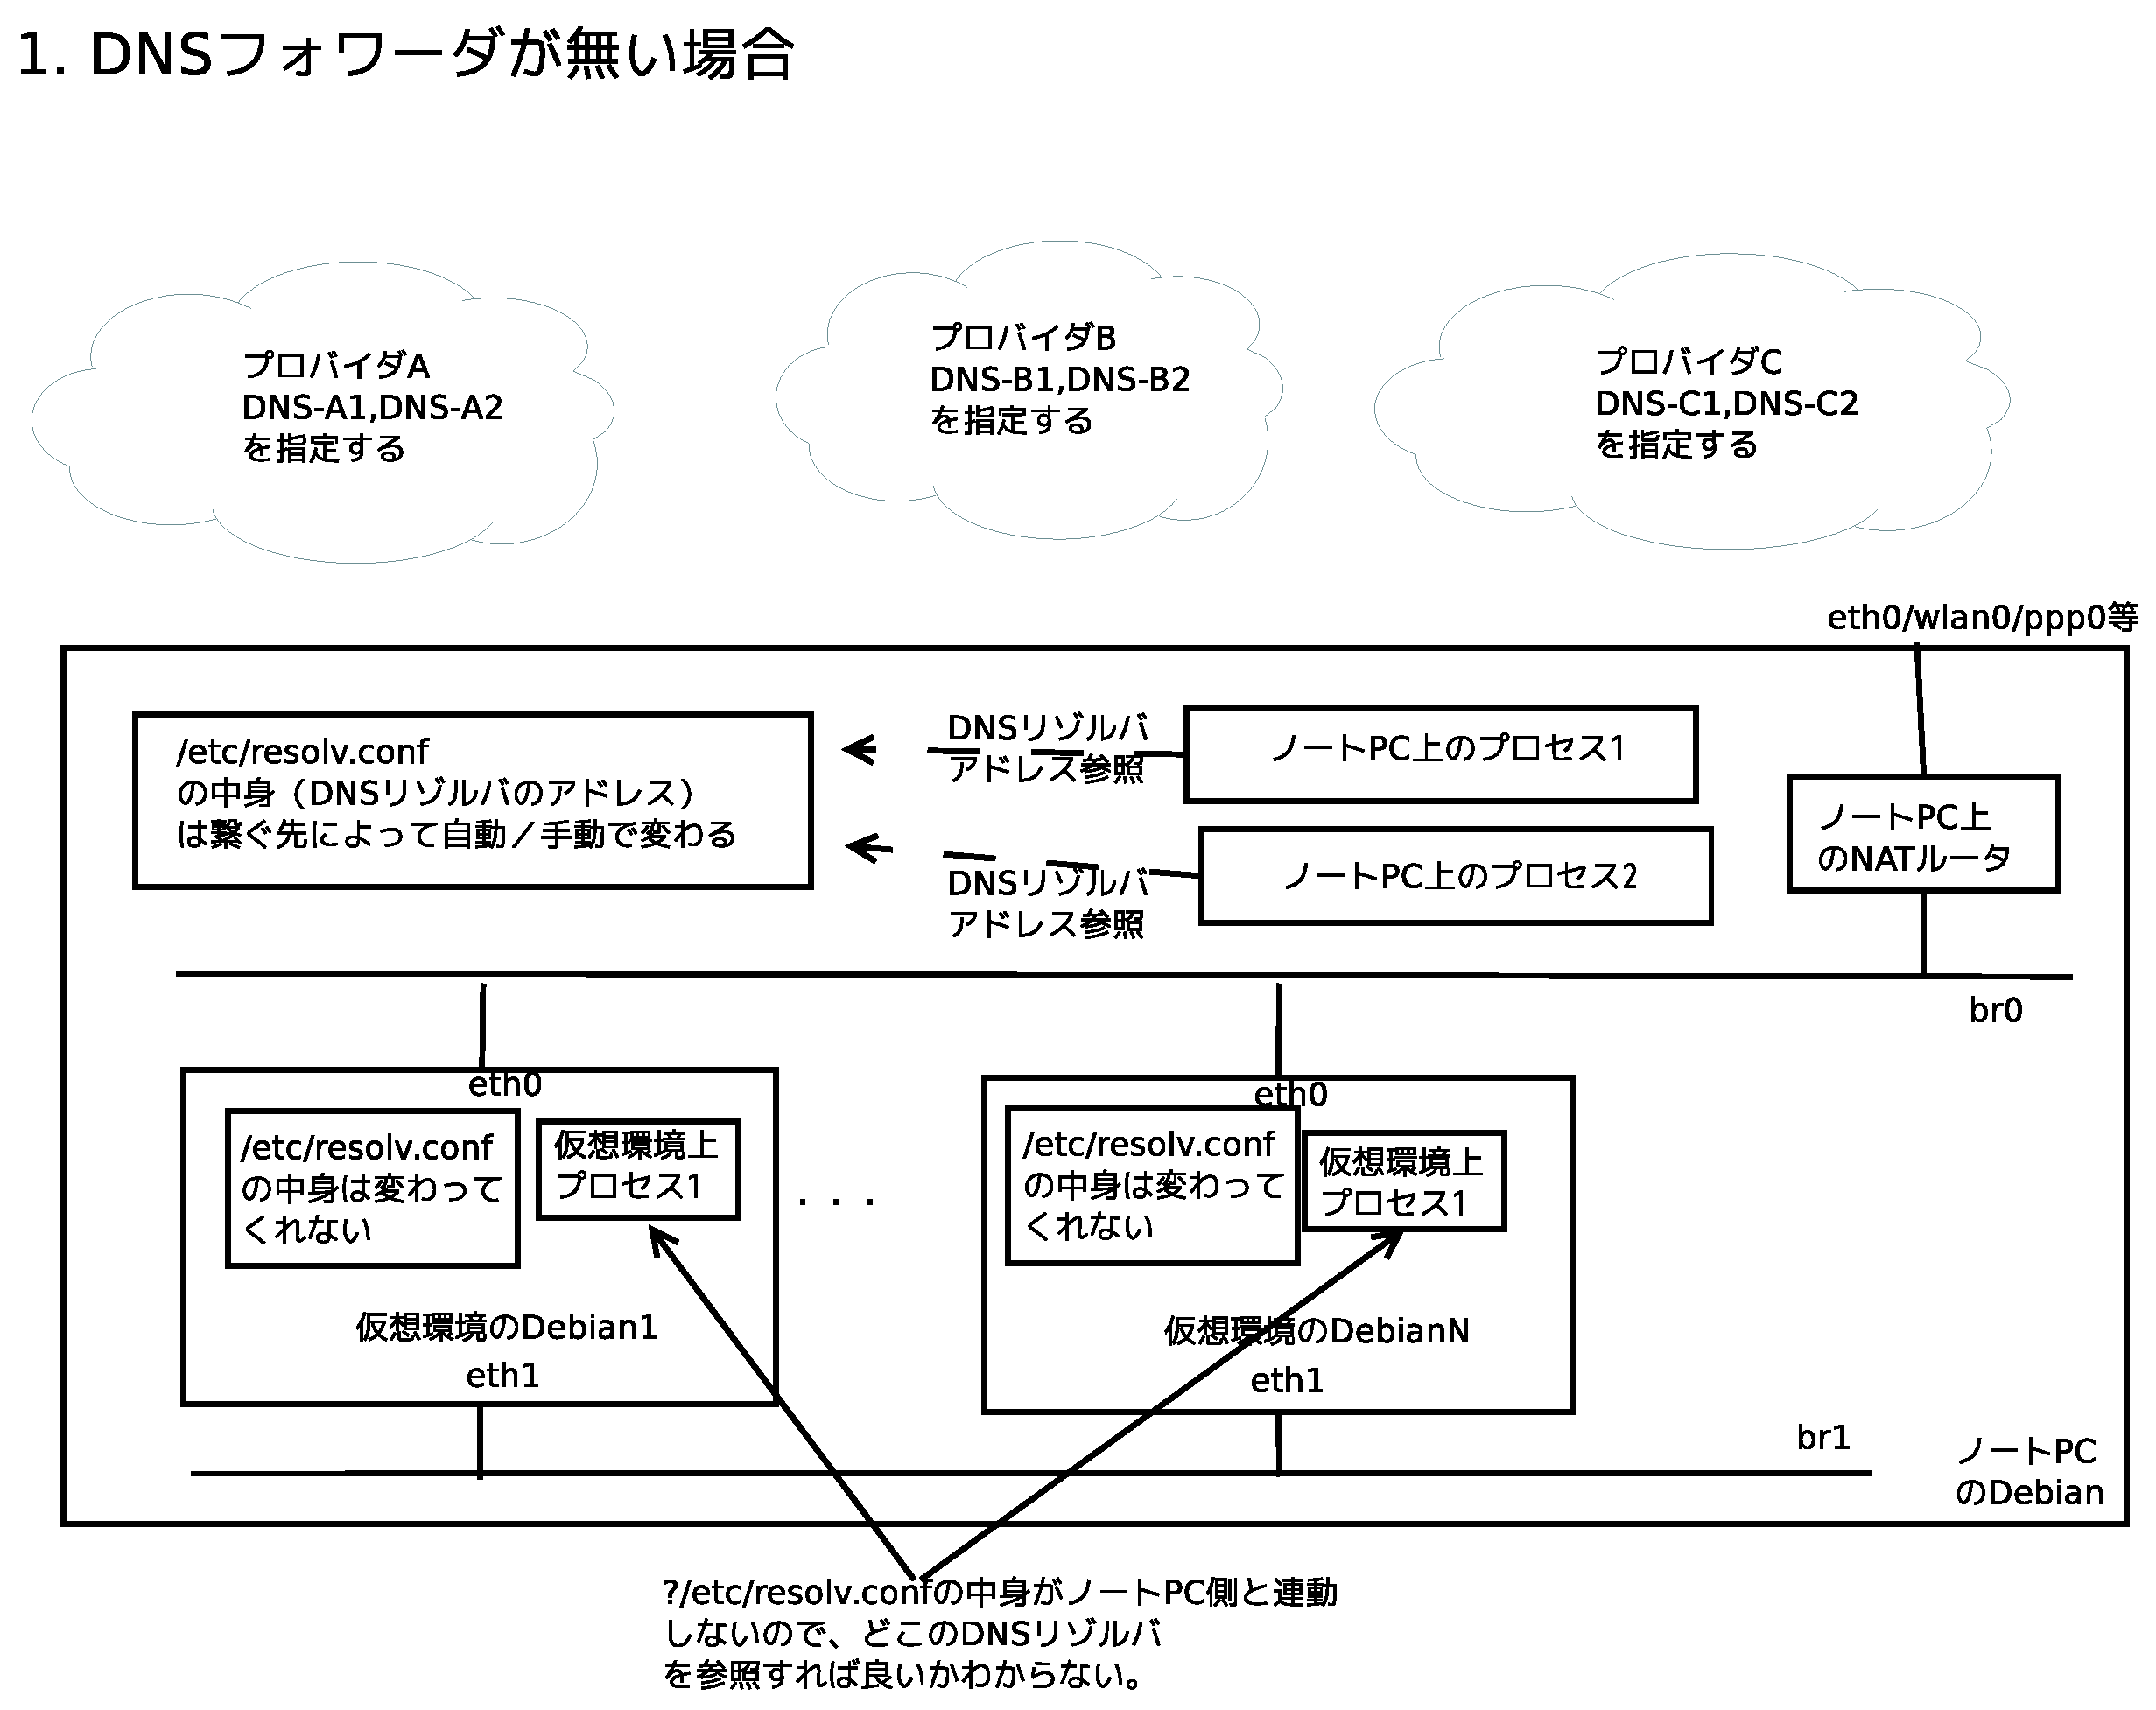
\includegraphics[width=0.5\hsize]{image201402/vm-dns-env.eps}
 \caption{dnsフォワーダが無い場合}\label{fig:vm-env1}
\end{center}
\end{figure}

\begin{figure}[H]
\begin{center}
 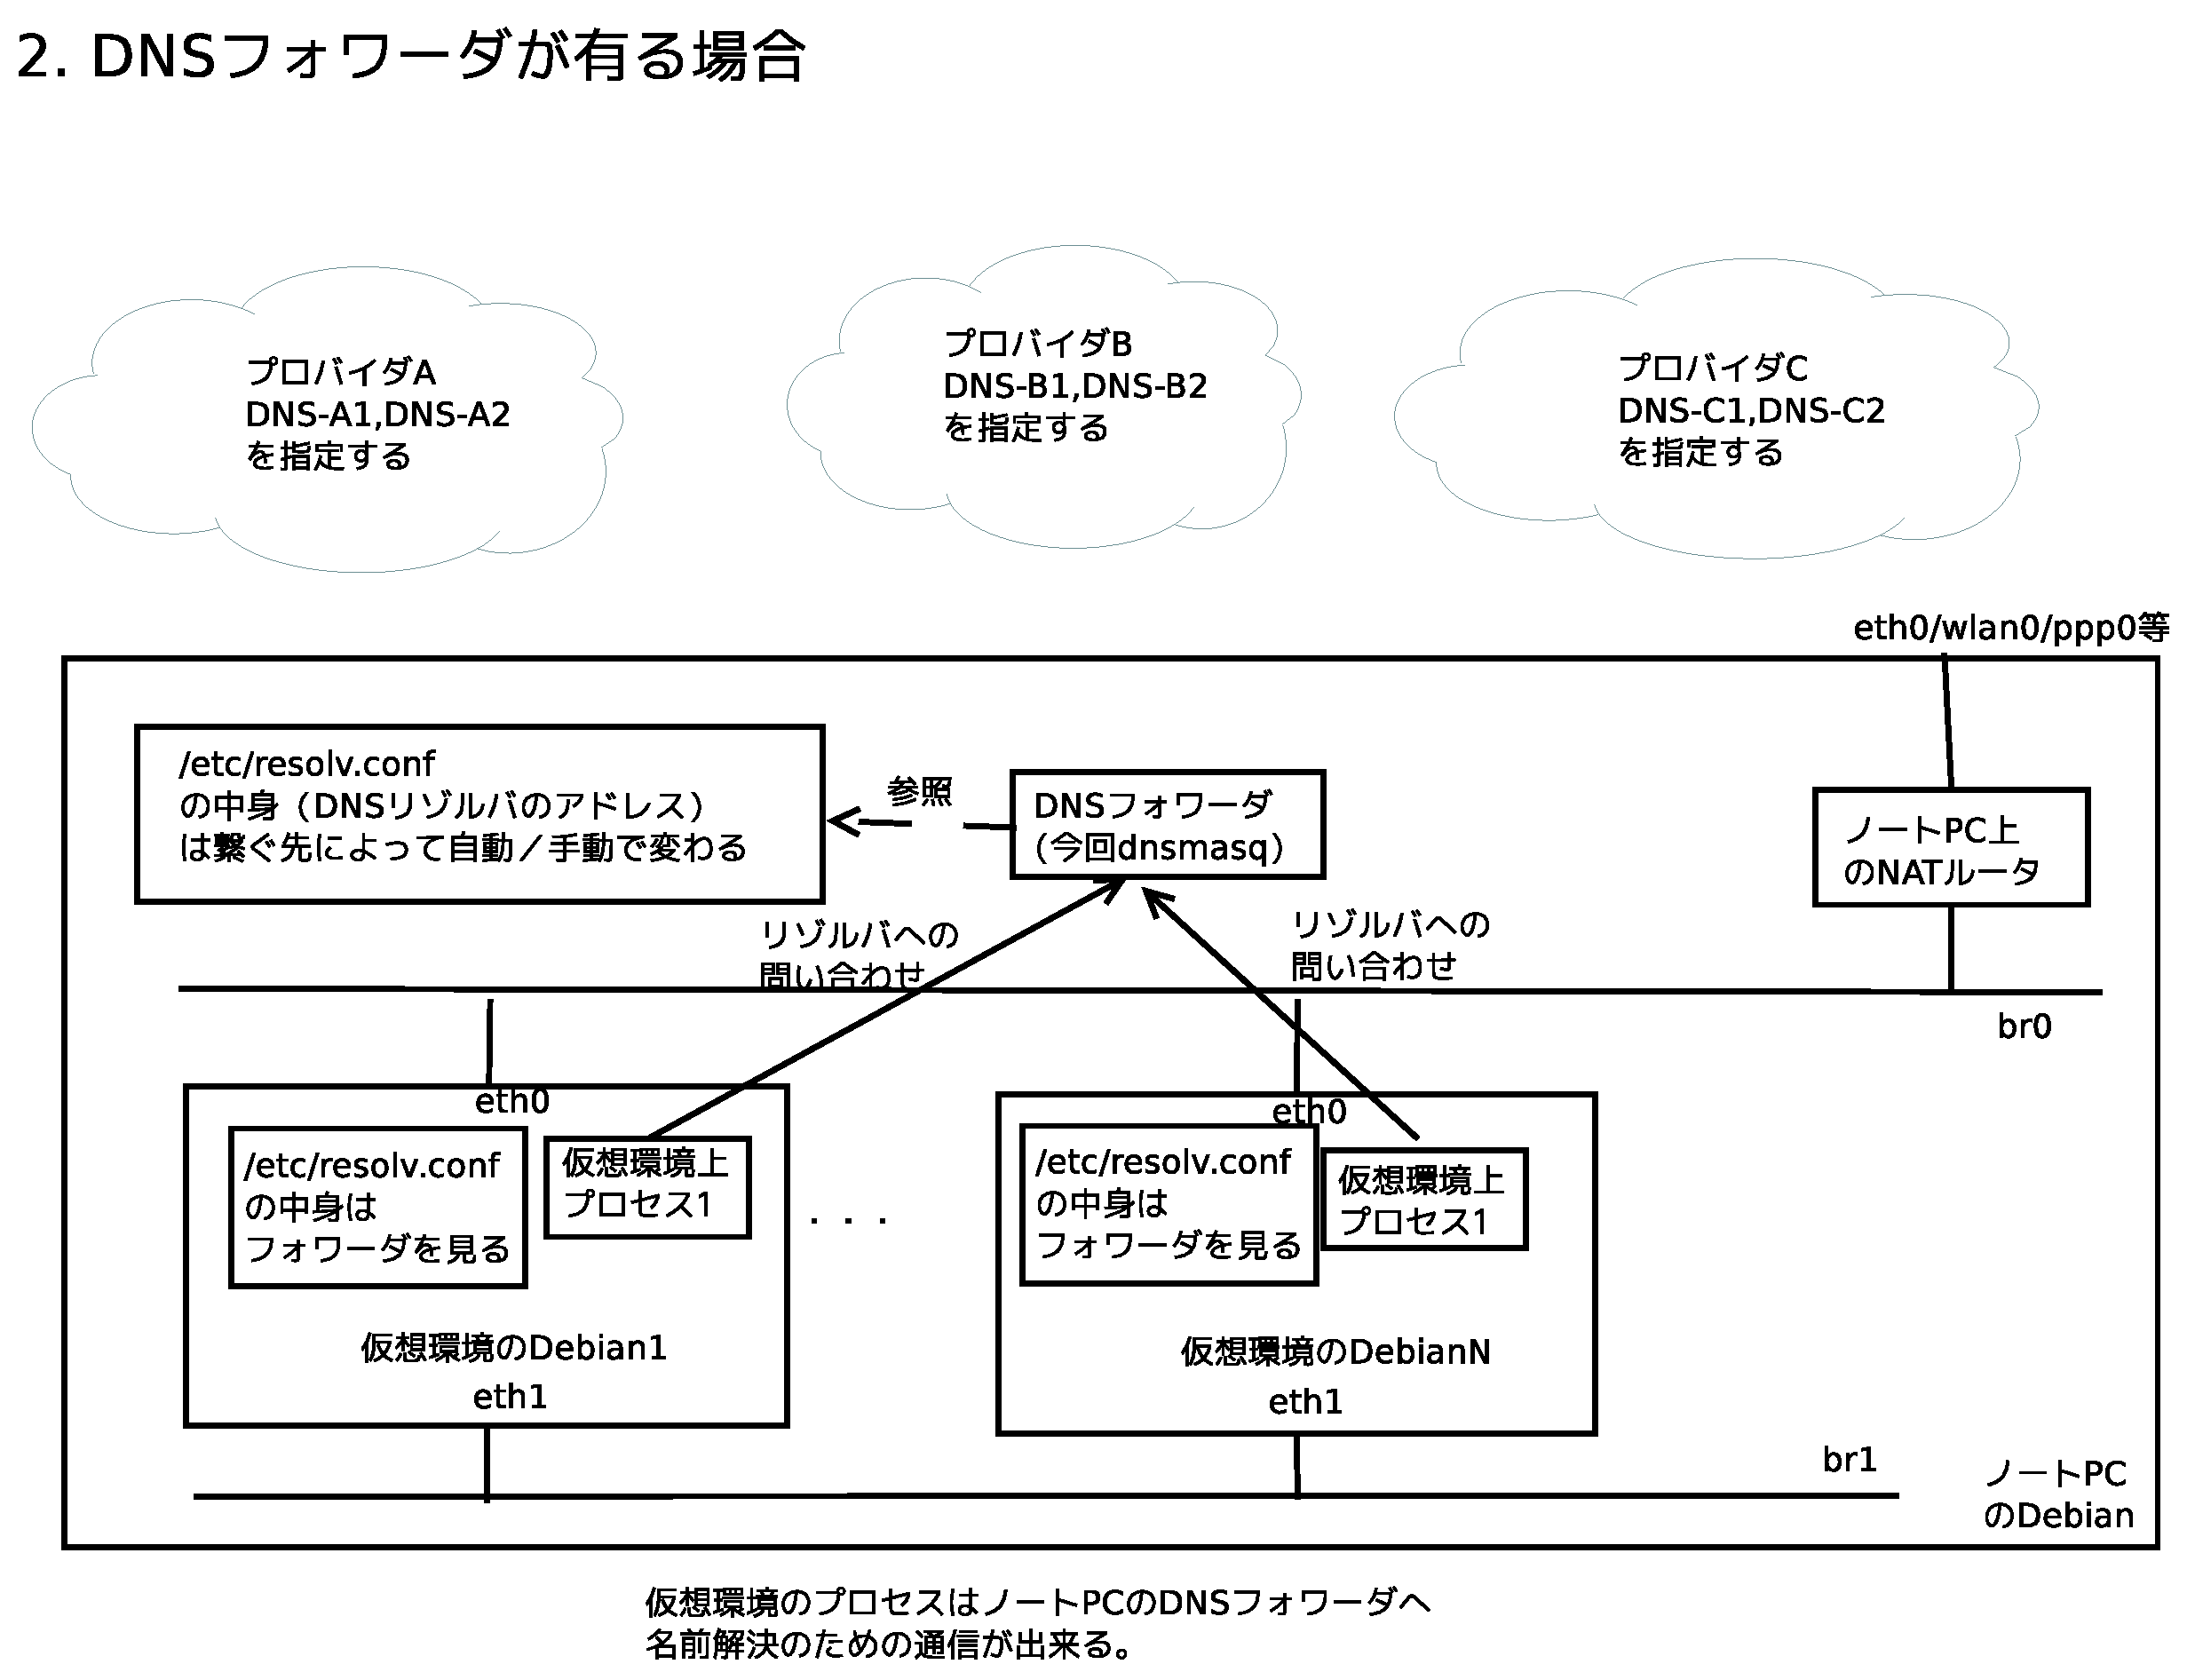
\includegraphics[width=0.5\hsize]{image201402/vm-dns-env2.eps}
 \caption{dnsフォワーダがある場合}\label{fig:vm-env2}
\end{center}
\end{figure}

 では早速使ってみます。

\begin{description}
\item[Step 1.] dnsmasqを導入します。
\begin{commandline}
note-pc$ sudo aptitude install dnsmasq
\end{commandline}
%$
\item[Step 2.] br0のみlistenするようにし、dnsフォワーダとしてのみ動作するように設定します。
\begin{commandline}
note-pc$ sudo vi /etc/dnsmasq.d/forwarder.conf
interface=br0
no-dhcp-interface=br0
bind-interfaces
\end{commandline}
%$

\item[Step 3.] dnsmasqをリスタートします。
\begin{commandline}
note-pc$ sudo service dnsmasq restart
\end{commandline}
%$

\item[Step 4.] 動作を確かめます
\begin{commandline}
特定のポートだけでListenしていることを確かめる
note-pc$ sudo netstat -nlp | fgrep dnsmasq
tcp  0 0 127.0.0.1:53  0.0.0.0:*   LISTEN      16955/dnsmasq   
tcp  0 0 192.168.0.1:53  0.0.0.0:* LISTEN      16955/dnsmasq   
udp  0 0 127.0.0.1:53    0.0.0.0:*             16955/dnsmasq   
udp  0 0 192.168.0.1:53  0.0.0.0:*             16955/dnsmasq   
実際にdnsmasqを指定して名前を引いてみる
note-pc$ sudo aptitude install dnsutils
note-pc$ dig @192.168.0.1 www.debian.org a
; <<>> DiG 9.9.3-rpz2+rl.13214.22-P2-Debian-1:9.9.3.dfsg.P2-4 <<>> @192.168.0.1 www.debian.org a
; (1 server found)
;; global options: +cmd
...中略...
;; ANSWER SECTION:
www.debian.org.		300	IN	A	5.153.231.4
www.debian.org.		300	IN	A	128.31.0.51
www.debian.org.		300	IN	A	130.89.148.14
...中略...
\end{commandline}
%$
\end{description}

非常に簡単にDNSフォワーダとしてセットアップ出来ます。

また、グローバル回線を変更した場合(例:拠点Aのwifiスポットから、拠点Bのwifiスポットへ移動した等)は、
\begin{commandline}
...グローバル回線を有効にして...
note-pc$ sudo service dnsmasq restart
\end{commandline}
%$
するだけで、新しいリゾルバ先をdnsmasqは取り込み、名前解決が出来るようになります。

\subsection{簡易DNSサーバーとして使う}

 今度は単一のドメインのホストレコードを返す簡単なDNSサーバーが
ちょっと欲しくなる時があります。このような場合、dnsmasqは
簡易DNSサーバーとしてもあっさり動作させることができます。

 実はdnsmasqはデフォルトで/etc/hostsを読み込み、DNSサーバーとしても
動作しています。そのため、簡易DNSサーバーとして利用する場合、
/etc/hostsをそのまま利用するのが一番簡単です。

\begin{description}
\item[Step 1.] /etc/hostsに名前解決したいホストを書きならべる。
\begin{commandline}
#例となります。
note-pc$ sudo vi /etc/hosts
-----------/etc/hostsここから---------------
192.168.0.3 debian0
192.168.0.4 debian1.my-domain debian1
192.168.0.5 debian2.my2-domain debian2
-----------/etc/hostsここまで---------------
\end{commandline}
%$
\item[Step 2.] dnsmasqをrestartします。
\begin{commandline}
note-pc$ sudo service dnsmasq restart
\end{commandline}
%$
\item[Step 3.] 実際にDNSを引いて確かめてみます。
\begin{commandline}
note-pc$ dig @192.168.0.1 debian0 +short
192.168.0.3 (←正しく返却されている)
note-pc$ dig @192.168.0.1 debian1.my-domain +short
192.168.0.4 (←正しく返却されている)
note-pc$ dig @192.168.0.1 debian2.my2-domain +short
192.168.0.5 (←上とは異なるドメイン所属のレコードも正しく返却されている)
note-pc$ dig @192.168.0.1 debian2 +short
192.168.0.5 (←ホスト名だけでも正しく返却されている)
\end{commandline}
%$
\end{description}

\subsection{簡易PXEブートをさせてみる}

 dnsmasqを使ってpxeブートを仮想化環境であるKVMから行ってみます。
ここでは、文献\cite{pxe-boot}の方法を使い、実際にwheezyのnetinst用
インストーラが立ち上がるまで確かめてみます。

\begin{description}
\item[Step 1.] /etc/dnsmasq.d/にて、今まで書いたファイルを一旦消去(適宜)
\begin{commandline}
note-pc$ sudo rm -f *
\end{commandline}
%$
\item[Step 2.] pxeboot用の定義を記載
\begin{commandline}
note-pc$ sudo vi /etc/dnsmasq.d/pxeboot.conf
----- pxeboot.confの中身-----
interface=br0
bind-interfaces
dhcp-range=192.168.0.129,192.168.0.254,255.255.255.0,1h
dhcp-boot=pxelinux.0,pxeserver
pxe-service=x86PC, "Install Linux", pxelinux
enable-tftp
tftp-root=/home/your/srv/tftp
----- pxeboot.confの中身-----
\end{commandline}
%$
\item[Step 3.] pxeブートさせるイメージを展開しておく。
\begin{commandline}
note-pc$ cd /home/your/
note-pc$ mkdir srv;mkdir tftp
note-pc$ cd srv/tftp
note-pc$ wget http://ftp.debian.or.jp/debian/dists/stable/main/installer-amd64/current/images/netboot/netboot.tar.gz
note-pc$ tar xzf netboot.tar.gz
\end{commandline}
%$
\item[Step 4.] dnsmasqを再起動
\begin{commandline}
note-pc$ sudo service dnsmasq restart
\end{commandline}
%$
\item[Step 5.] virt-installコマンド経由で、pxeブートしてみる。
\begin{commandline}
note-pc$ sudo qemu-img create -f raw /var/lib/libvirt/images/debian-pxe 5G
note-pc$ sudo virt-install --connect=qemu:///system -n debian-pxe --ram 512 \
           --pxe --disk /var/lib/libvirt/images/debian-pxe,bus=virtio,size=5,format=raw,cache=writeback \
           --bridge=br0,model=virtio --vnc --hvm --accelerate
\end{commandline}
%$
\end{description}

 virt-viewerがすぐに開き、PXEブートして、Debian wheezyのインストール画面が出てきます。

\subsection{終わりに}

 今回ここでは、簡易dnsフォワーダ、簡易dnsサーバー、簡易pxeサーバー
をdnsmasqを使って組み立てました。

 しかし、man dnsmasqを読むと判る通り、もっと複雑な事も簡単に出来ます。
また、自分はまったく未評価ですが、最近ではlua言語と合わせて使う事ができるようです。

 複数の仮想環境を使ってノートPC上に複数のDebianの開発環境を立ち上げる場合に、
非常に便利です。dnsmasqをぜひ一度お試しあれ。

\begin{thebibliography}{0}
  \bibitem{kde-devel-debian}
    {\footnotesize{
       野島 貴英,「Debian開発者のKDE環境あれこれ」,第85回東京エリアDebian勉強会資料,
       \url{http://tokyodebian.alioth.debian.org/pdf/debianmeetingresume201202.pdf}
       }}
  \bibitem{pxe-boot}
    {\footnotesize{
       Debian.org,``PXEBootInstall'',
       \url{https://wiki.debian.org/PXEBootInstall}
       }}
\end{thebibliography}

201403 tokyo
%-------------------------------------------------------------------------------
\dancersection{Debianでiphone5を繋ぐ}{野島 貴英}
%-------------------------------------------------------------------------------
\index{debian-iphon5}

\subsection{はじめに}

 大変不自由なスマートフォンなのに日本で驚異的に売れまくっているという、目を
被いたくなるような現実を作り出しているスマートフォンの1つとして、
iphone5があります\cite{iphone-japan-share}。このスマートフォン、
PCに繋ぐには、windows/macでiTuneなどの専用プロプリエタリなソフトウェアを
使ってデータ同期をしなければならないという、これでもかというぐらいの
不自由仕様となっています。

 ここでは、少しでもiphone5の不自由さを回避するため、

\begin{itemize}
\item 自由なDebianマシンに、なんとかして不自由なiphone5を繋ぐ事について、
\item iphone5がどのような仕組みでつながるのか(Debian開発者向け)
\end{itemize}

について述べます。

\subsection{本発表内容についての情報ソース}

 本発表内容の技術の情報ソースは、すべて

\begin{itemize}
\item Apple社のディベロッパーサイトで公開情報となっているもの(文献\cite{apple-fs-program-ref})
\item Debianパッケージに含まれるプログラムを解析した範囲
\item その他Webにて公開されている情報(文献\cite{usb-mux-desc},\cite{afc-desc},
\cite{iphone-hacking-accessories-desc})
\end{itemize}

のみに基づきます。

\subsection{Debianに繋ぐ}

 東京エリアDebian勉強会にいらっしゃるような方々は、普段から
Debian sidをお使いかと思いますので、ここでは、Debian sid
を用い、さらにパッケージのバージョンが低くて問題のある部分だけちょっと自作して
\footnote{すみません、bug reportあげときます...}繋ぐ方法を取ってみます。

 まずは、用意するものを表\ref{tab:iphone5-debian-prerequisite}に記載します。

\begin{table}[ht]
\begin{center}
\begin{tabular}{|l|p{7cm}|l|}
\hline 
項番 & 品目 & 備考 \\ \hline
1 & Debian sidの入っているマシン & \\ \hline
2 & iphone5 & iOS7.1(3/14現在最新)にバージョンアップ済み \\ \hline
3 & Lightning-USBケーブル & \\ \hline
4 & Debianと繋ぐ先のiphoneアプリ。なんでも良いかと思いますが、ここではファイルマネージャアプリであるDocument 2 Free を例にあげます。& \\ \hline
\end{tabular}
\caption{用意するもの}\label{tab:iphone5-debian-prerequisite}
\end{center}
\end{table}

\begin{description}
\item [Step 1.] iphone5にDocument 2 Free\footnote{\url{https://itunes.apple.com/us/app/documents-2-free-file-manager/id314894105}}をインストールしておきます。
\item [Step 2.] debian sidで導入されるlibmobiledevice4のupstreamバージョンが古く、iOS7.1に対応出来ないので、upstream最新版からパッケージを自作して最新のものにします。
\begin{commandline}
$ sudo aptitude install git
$ git clone https://github.com/libimobiledevice/libimobiledevice.git libimobiledevice-1.1.6
$ mkdir libimobiledevice4
$ cd libimobiledevice4
# Debianで用意されているlibimobiledeviceに梱包されているdebianディレクトリを利用
$ apt-get source libimobiledevice4/sid
$ cd libimobiledevice-1.1.5
$ cp -a debian ../../libimobiledevice-1.1.6
$ cd ../../libimobiledevice-1.1.6
# いろいろパッチを当てる
# 主に、libimobiledevice-1.1.6だと1.1.5用のパッチはupstreamで適用済みなのではずす、
# docパッケージの中身は作り方が違う、一部シンボルテーブルも違うなどで
# チェックを除外するのが目的。
$ rm -f debian/libimobiledevice-doc.doc-base
$ rm -f debian/libimobiledevice-doc.install
$ rm -f debian/libimobiledevice-doc.links
$ rm -f debian/libimobiledevice4.symbols
$ rm -rf debian/patches
\end{commandline}
\begin{commandline}
$ patch -p1 <<__HERE
diff -ur a/debian/changelog b/debian/changelog
--- a/debian/changelog  2013-10-30 02:42:24.000000000 +0900
+++ b/debian/changelog  2014-03-13 21:50:16.000000000 +0900
@@ -1,3 +1,9 @@
+libimobiledevice (1.1.6-1~a1) unstable; urgency=low
+
+  * update latest upstream
+
+ -- Your Name <your@mail.addr>  Fri, 28 Feb 2014 01:42:21 +0900
+
 libimobiledevice (1.1.5-2) unstable; urgency=low
 
   * [0052e46] Drop hal fdi file.
diff -ur a/debian/control b/debian/control
--- a/debian/control    2013-10-30 02:42:24.000000000 +0900
+++ b/debian/control    2014-02-28 01:42:09.000000000 +0900
@@ -102,13 +102,3 @@
  .
  This package contains utilities and examples which use libimobiledevice.
 
-Package: libimobiledevice-doc
-Architecture: all
-Section: doc
-Depends: libjs-jquery, ${misc:Depends}
-Description: Library for communicating with iPhone and iPod Touch devices
- libimobiledevice is a library that talks the native Apple USB protocols that
- the iPhone and iPod Touch use. Unlike other projects, libimobiledevice does
- not depend on using any existing libraries from Apple.
- .
- This package contains the documentation for the library.
diff -ur a/debian/rules b/debian/rules
--- a/debian/rules      2013-10-30 02:42:24.000000000 +0900
+++ b/debian/rules      2014-02-28 01:49:58.000000000 +0900
@@ -25,7 +25,7 @@
        rm -rf $(CURDIR)/debian/tmp//usr/lib/python*/dist-packages/*.a
        #Remove installed man pages, installed by *.manpages
        rm -f $(CURDIR)/debian/tmp/usr/share/man/man1/*.1
-       dh_install --fail-missing
+       dh_install 
 
 override_dh_strip:
        dh_strip --dbg-package=libimobiledevice4-dbg
@@ -34,5 +34,3 @@
        # Only build for the current version of python, not all supported.
        dh_python2 --no-guessing-versions
 
-override_dh_makeshlibs:
-       dh_makeshlibs -- -c4
__HERE
$ sudo aptitude build-dep libimobile4/sid
$ debuild -uc -us
$ cd ..
$ sudo dpkg -i ./libimobiledevice4_1.1.6-1~a1_amd64.deb ./libimobiledevice-utils_1.1.6-1~a1_amd64.deb
\end{commandline}
%$
\item [Step 3.] 他にiphone5に繋ぐための必要なパッケージを導入しておきます。
\begin{commandline}
$ sudo aptitude install ideviceinstaller ifuse 
...いろいろ依存関係に引きずられて入る...
\end{commandline}
%$
\item [Step 4.] Debianマシンにて、fuseグループにユーザを追加し、一旦ログアウト&ログイン操作を行います。(ログアウト&ログイン操作を行う事が重要です)
\begin{commandline}
$ sudo usermod -a -G fuse <your-login-id>
$ exit (あるいは、デスクトップ環境のログアウト操作)
your machine login: <your-login-id>
Password: ...your pass...
(あるいは、デスクトップ環境のログイン操作)
$ 
\end{commandline}
%$
\item [Step 5.] iphone5のロック画面を解除し、Lightning-USBケーブルでDebianマシンと繋ぎます。
\item [Step 6.] Debian側、iphone5側両方に「コンピュータ/デバイスを信頼するか?」という意味のポップアップが表示されるかもしれませんが、「信頼する」を押して一旦抜けます。
\item [Step 7.] iphone5とペアリングを行います。
\begin{commandline}
$ sudo idevicepair pair
SUCCESS: Paired with device ...40桁のuuid...
\end{commandline}
%$
なお、この時、iphone5に「コンピュータを信頼しますか?」というポップアップが出るので、「信頼する」を選択します。すると、Debian機材の/var/lib/lockdown/以下に必要ファイルができる。以降はidevicepair操作を行わなくてもiphone5との通信が出来るようになります。
\item [Step 8.] iphone5にすでにインストールされているアプリケーションのappidをDebianから探します。こちらの結果から、Document 2 Freeのappidはcom.savysoda.documents2Freeである事が分かります。
\begin{commandline}
$ ideviceinstaller -l
Total: 16 apps
com.savysoda.documents2Free - Documents 2 7.3
com.square-enix.gunsandsouls - GUNS 1.0.1
com.google.b612 - Google Earth 7.1.1
...中略...
\end{commandline}
%$
\item [Step 9.] Document 2 Freeのストレージをマウントし、本勉強会資料を投げ込んでみます。(もちろん、動画ファイルとか、mp3ファイルとか投げ込んでも問題ありません)
\begin{commandline}
# マウントポイント作ってifuseでマウントする。
$ mkdir document2
$ ifuse --appid com.savysoda.documents2Free `pwd`/document2
$ cd document2
# document2 Freeのストレージが見える
$ ls -l
Inbox/ mraid.js 
$ mkdir 東京Debian
$ cp /home/yours/doc/monthly-report/debianmeetingresume201403.pdf 東京Debian/
$ cd ..
# unmountはfusermountコマンドを使う。
$ fusermount -u `pwd`/document2
\end{commandline}
\item [Step 10.] iphone5側でDocument 2 Freeを立ち上げると、東京Debianというフォルダが出来ており、さらにその下にpdfファイルが見えます。こちらをタップすると、本資料をiphone5上で読むことが出来ます。
\end{description}

\subsection{仕組み}

 東京エリアDebian勉強会に集まるような人にとっては、ただ繋ぐだけではおもしろくないと思いますので、仕組みについて説明します。

\subsubsection{iphoneアプリのストレージの約束事}

 iphoneアプリは、apple社が定めるいろいろな約束ごとに基づいて設計されています。

 今回マウントしたiphoneアプリのストレージに関する約束ごとは、公開情報となっているApple Developerサイト掲載の「ファイルシステム プログラミングガイド」\cite{apple-fs-program-ref}に詳細があります。この中で、知っておくべき事として、

\begin{itemize}
\item iphoneアプリは各々割り当てられたサンドボックス内のリソースでしか動作を許されていません。そのため、例えばAアプリからBアプリのストレージ領域をアクセスすることがそもそも出来ません。
\item ディレクトリの名前と用途が統一的に決められています。(例:Documents/,Library/,tmp/)
\end{itemize}

となっています(図\ref{fig:iphone-app-fs-overview}参照。) 今回マウントに利用したifuseコマンドですが、このコマンドは、通常は
オプション--appidで指定したiponeアプリの持つDocumentsディレクトリをマウントする能力があります。
(注:所謂jail breakしたiphone端末は除きます)

\begin{figure}[H]
\begin{center}
 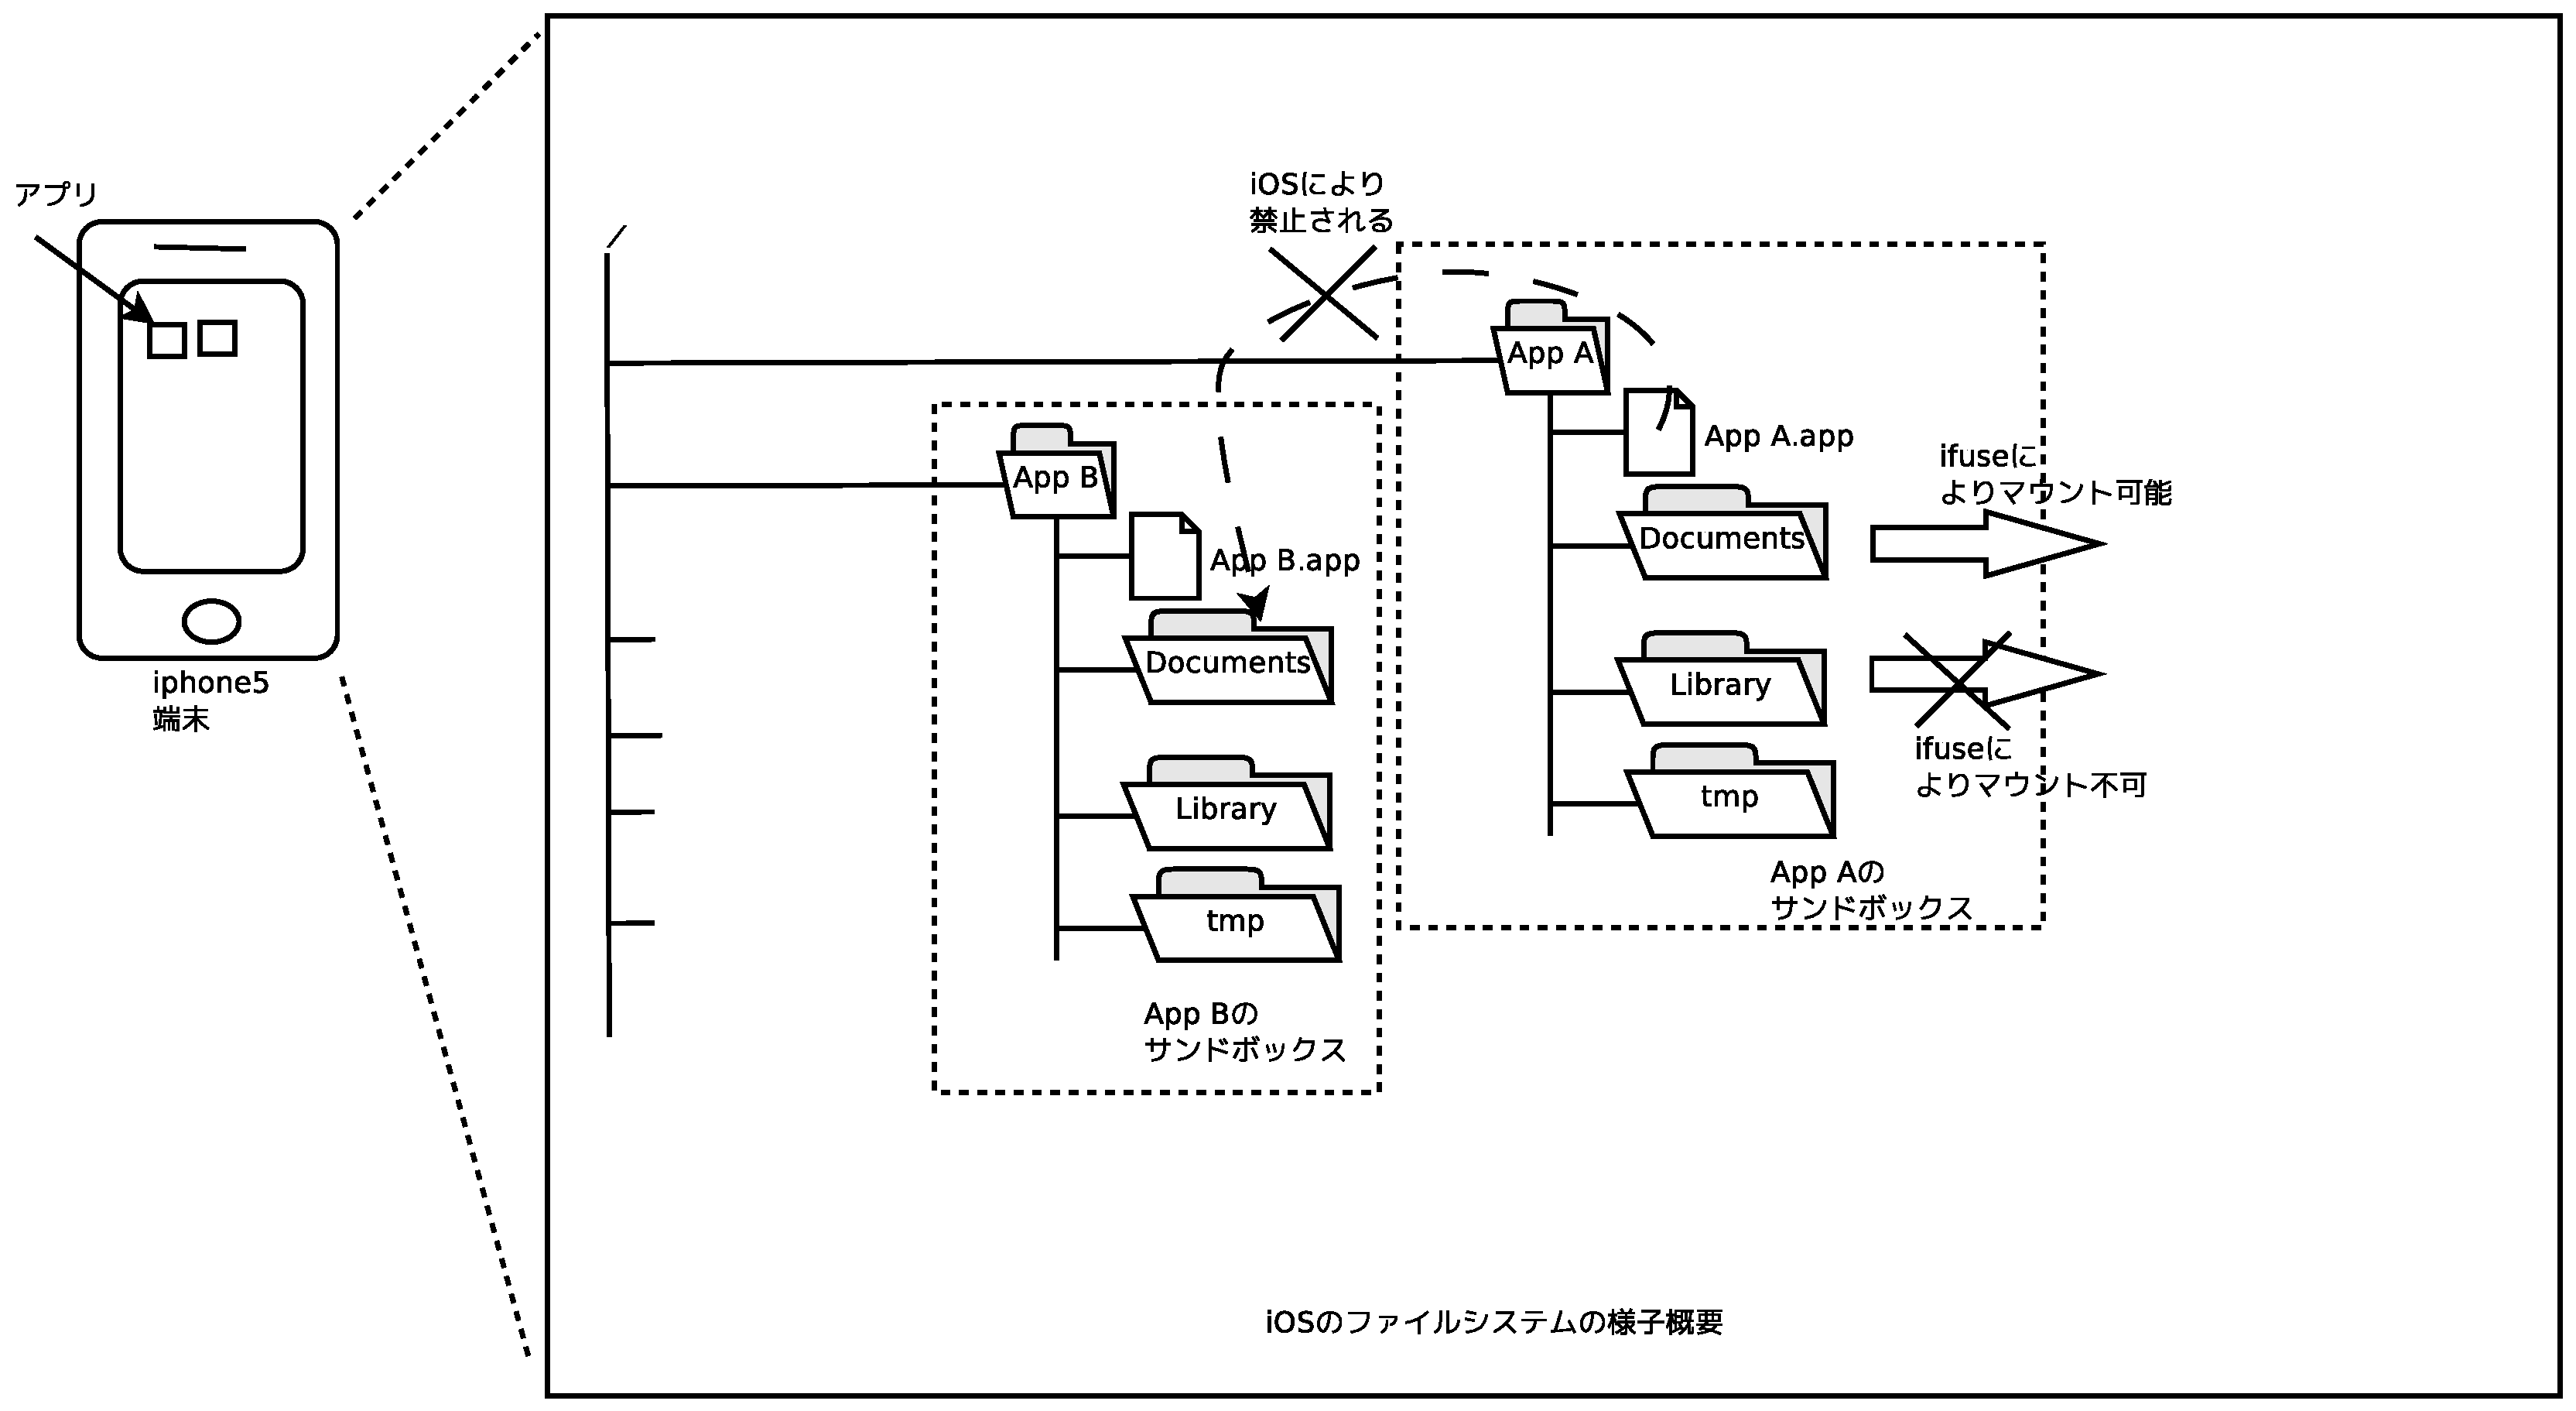
\includegraphics[width=0.8\hsize]{image201403/iphone-app-fs-overview.eps}
 \caption{iphoneアプリのストレージの様子}\label{fig:iphone-app-fs-overview}
\end{center}
\end{figure}

\subsubsection{Debianとの通信の仕組み}

 今回紹介の件についてiphone5とDebianとの通信の仕組みを図\ref{fig:iphone-communication-diagram}に示します。

\begin{figure}[H]
\begin{center}
 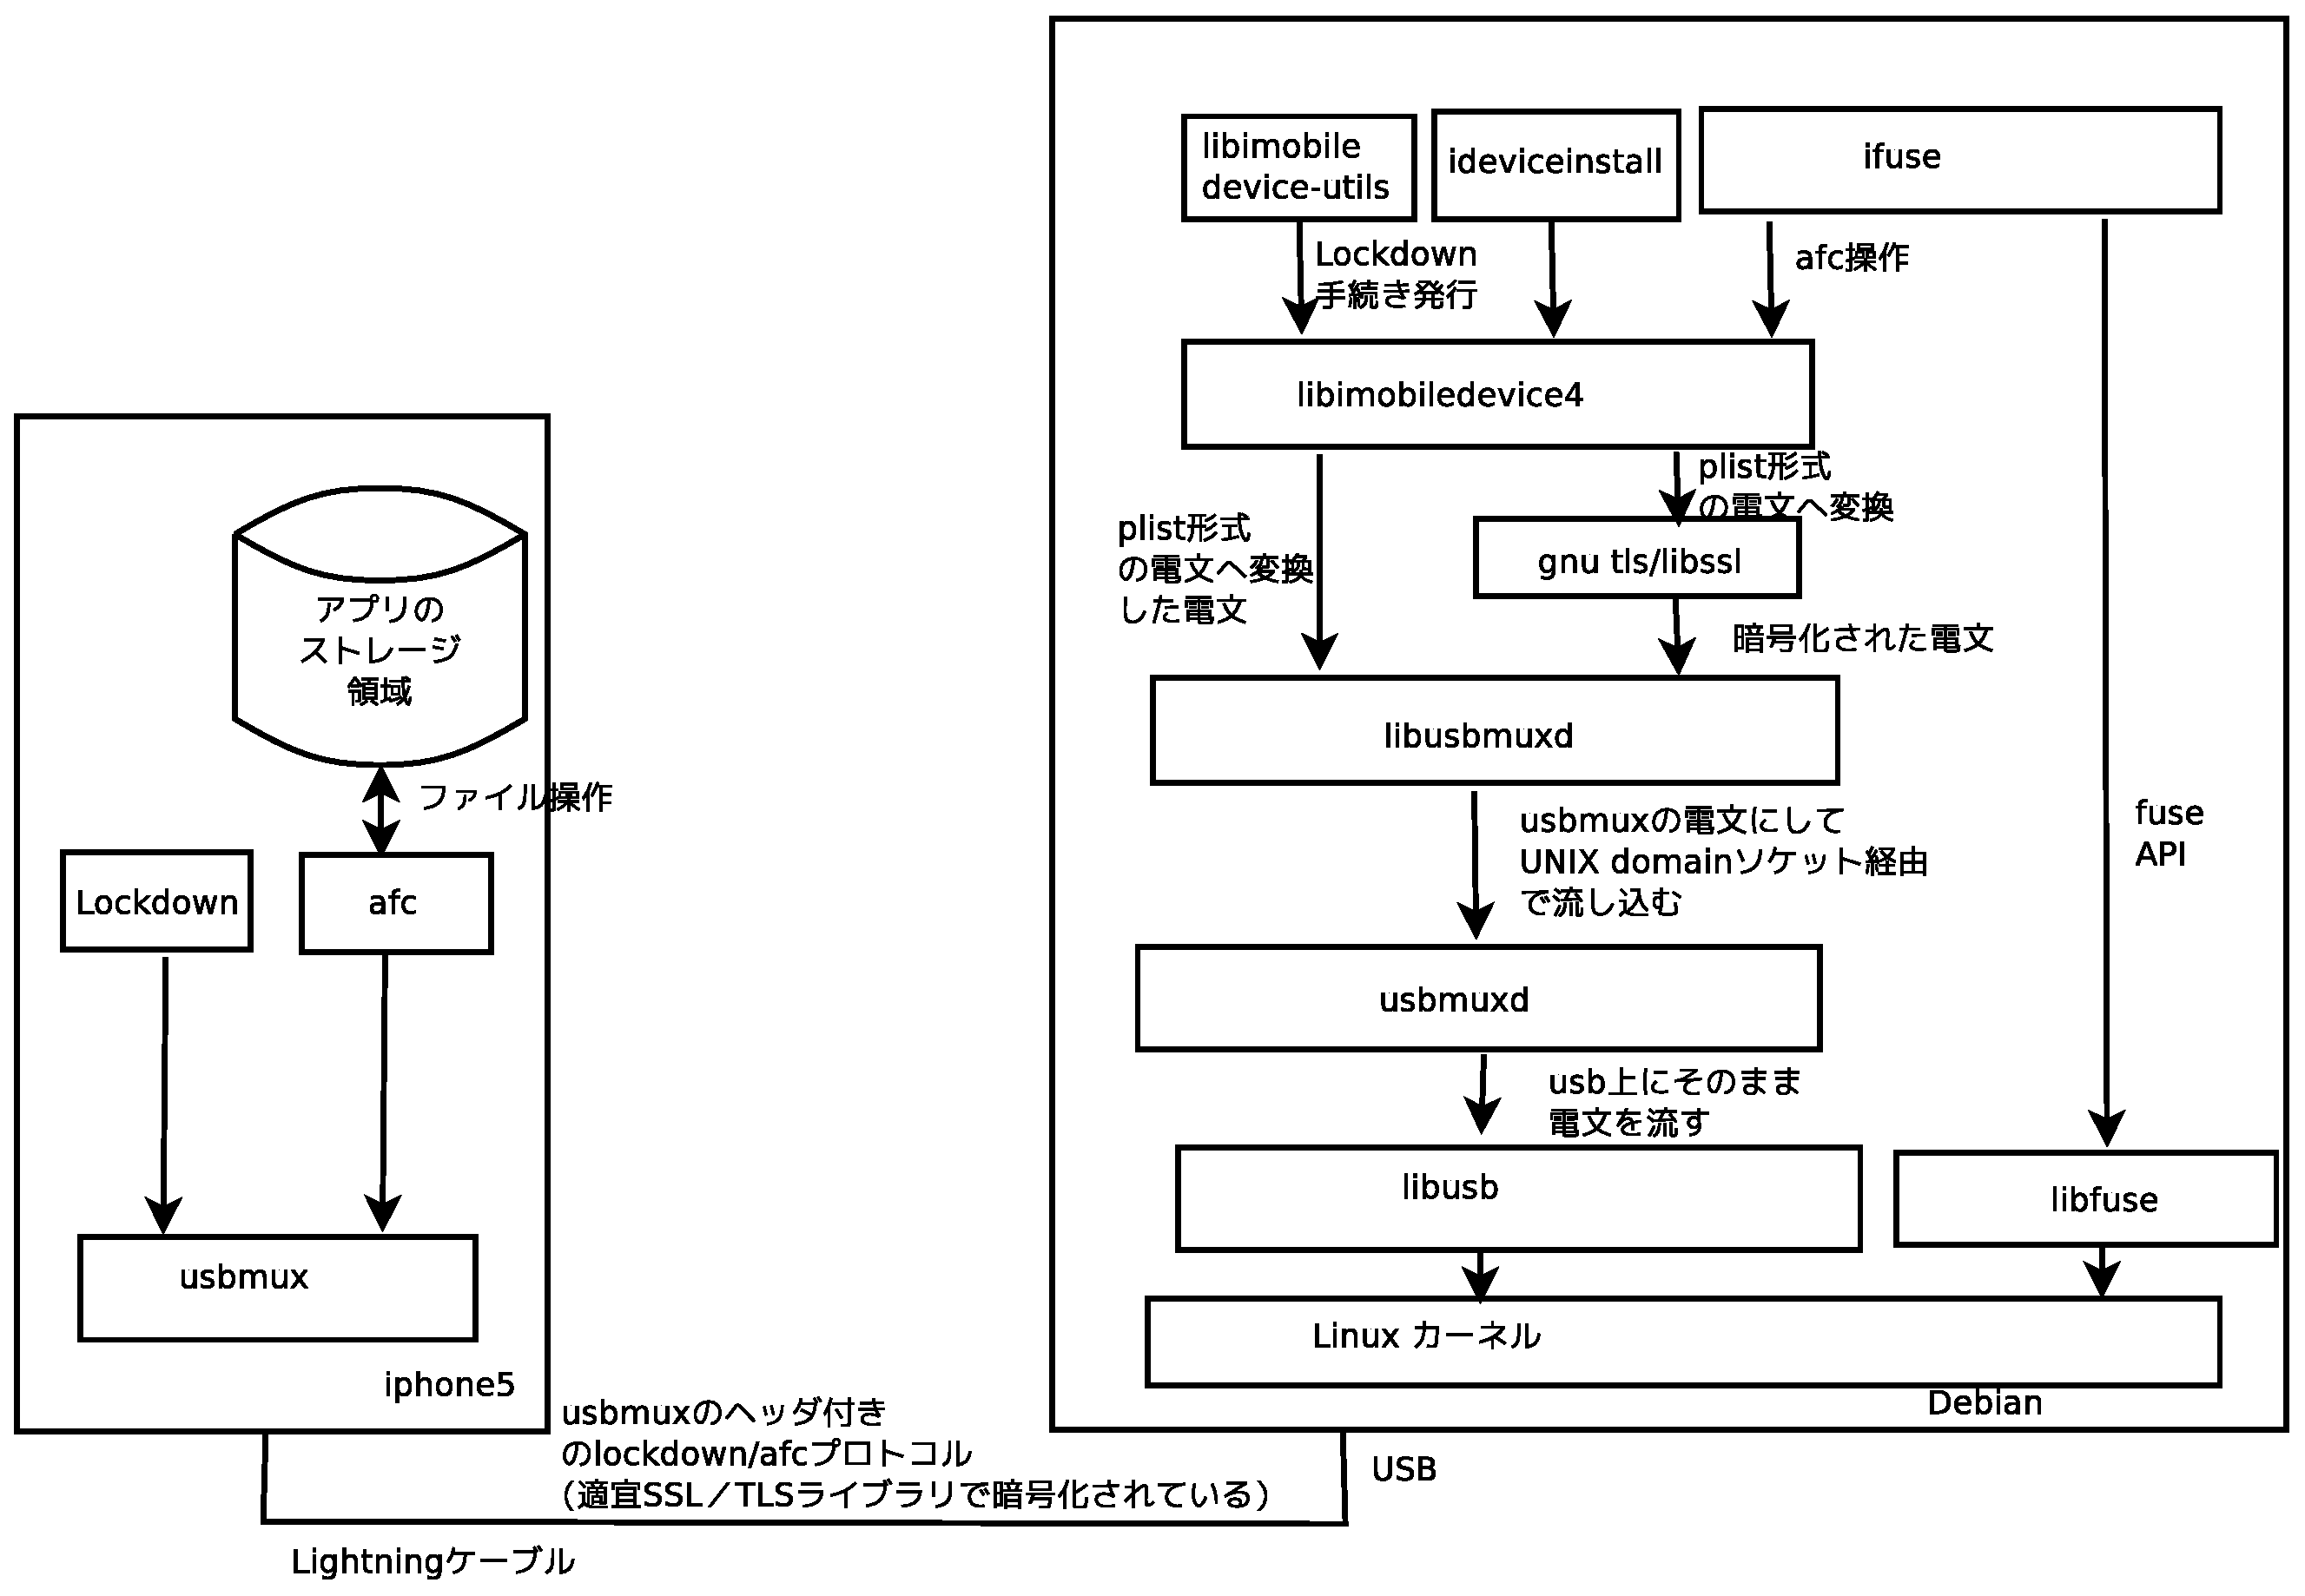
\includegraphics[width=0.8\hsize]{image201403/iphone-communication-diagram.eps}
 \caption{iphone5とDebianの通信の仕組み}\label{fig:iphone-communication-diagram}
\end{center}
\end{figure}

 基本的に、Lightning-USBケーブル上には、usbmuxのパケットが流れます。
 さらにペイロードとして、lockdownプロトコルと言われるプロトコル、afcプロトコルが適宜SSL/TLSライブラリ
で暗号化されて乗っています。

 プロトコルについて階層化して図示すると図\ref{fig:iphone-protocol-layerd}に示します。

\begin{figure}[H]
\begin{center}
 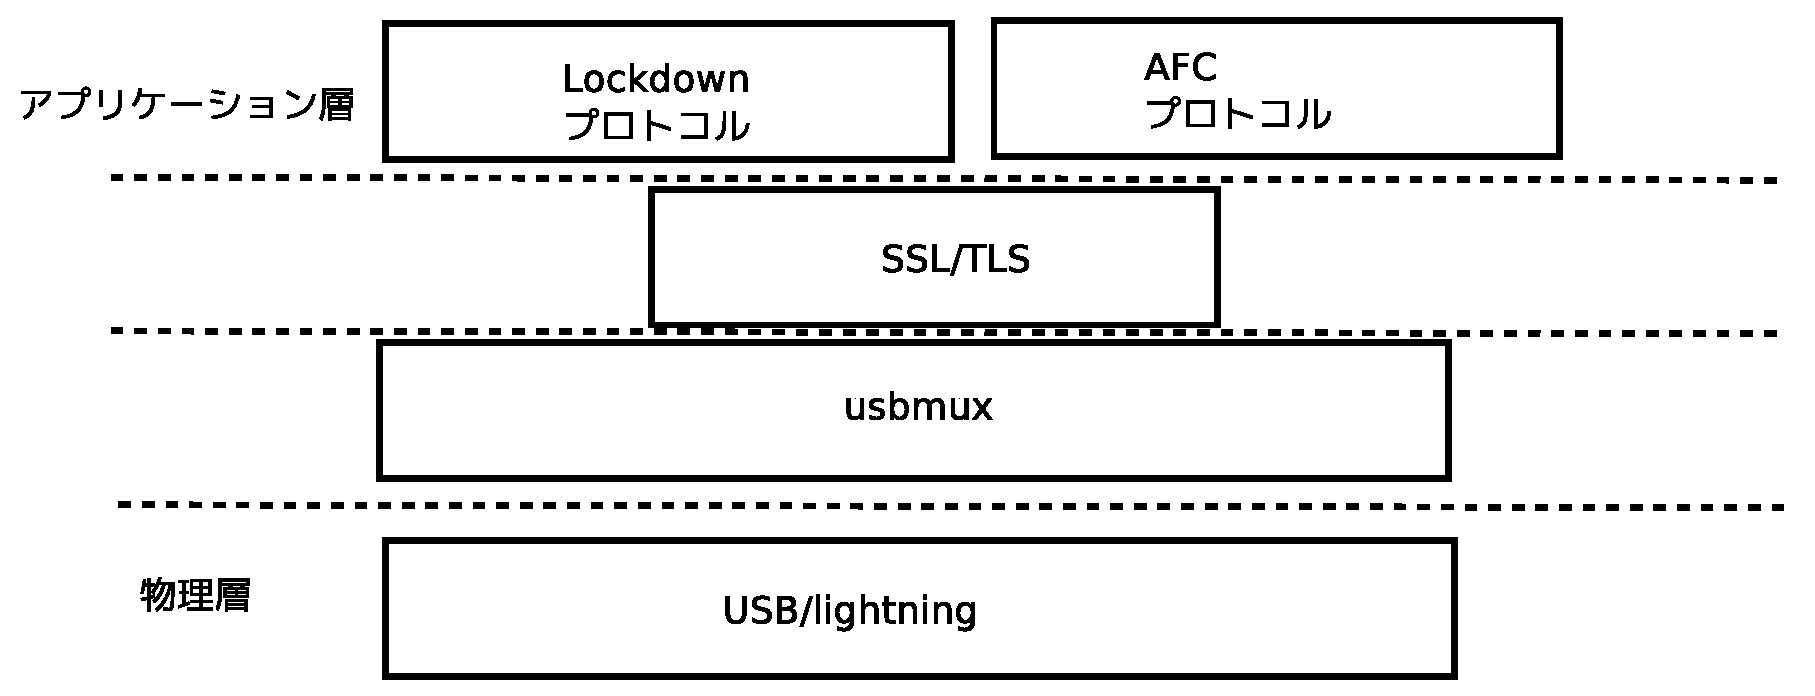
\includegraphics[width=0.8\hsize]{image201403/iphone-protocol-layerd.eps}
 \caption{iphone5との通信プロトコル}\label{fig:iphone-protocol-layerd}
\end{center}
\end{figure}

 また、各々のプロトコルについての説明を表に示します。

\begin{table}[ht]
\begin{center}
\begin{tabular}{|l|l|p{7cm}|}
\hline 
項番 & プロトコル名 & 概要 \\ \hline
1 & usbmux & lightning/usbに流れているプロトコル\\ \hline
2 & Lockdown & iphone5との通信認証、iphone5のLightning端子側から利用出来るサービスのやりとりを担当。plist形式の電文をusbmuxに載せ、iphone5とやりとりを行う。 \\ \hline
3 & afc & Apple File Connectionのためのプロトコル。ファイルシステム操作が出来る。\\ \hline
\end{tabular}
\caption{プロトコル名称と概要}\label{tab:iphone5-protocol-overview}
\end{center}
\end{table}

 また、plist形式とは、property listの略で、バイナリ形式の電文と、XML形式の電文の2種類があるようです。

 なお、電文のやりとりの詳細、電文の説明については、文献\cite{usb-mux-desc},\cite{afc-desc},
\cite{iphone-hacking-accessories-desc}に詳細があります。

\subsection{終わりに}

 今回、Debianにiphone5を繋ぎ、iTuneによらないデータ転送について紹介しました。また、
実現する技術についても紹介しました。こちらにより、不自由なスマートフォンを少しでも自由に使う事が
出来れば幸いです。

\begin{thebibliography}{0}
  \bibitem{iphone-japan-share}
    {\footnotesize{
       GIGAZINE,「Appleが過去最高の売上を発表、日本ではiPhoneが69\%のシェアを獲得」,
       \url{http://gigazine.net/news/20140128-apple-report-fy14-q1/}}}
  \bibitem{apple-fs-program-ref}
    {\footnotesize{
       Apple Developerサイト,「ファイルシステム プログラミングガイド」,
       \url{https://developer.apple.com/jp/devcenter/ios/library/japanese.html}}}
  \bibitem{usb-mux-desc}
    {\footnotesize{
       theiphonewiki,``Usbmux'',
       \url{http://theiphonewiki.com/wiki/Usbmux}}}
  \bibitem{afc-desc}
    {\footnotesize{
       theiphonewiki,``afc'',
       \url{http://theiphonewiki.com/wiki/AFC}}}
  \bibitem{iphone-hacking-accessories-desc}
    {\footnotesize{
       GOTO:Hack,``Hacking apple accessories to pown iDevices'', Mathieu RENARD,
       \url{http://2013.hackitoergosum.org/presentations/Day3-04.Hacking%20apple%20accessories%20to%20pown%20iDevices%20%E2%80%93%20Wake%20up%20Neo!%20Your%20phone%20got%20pwnd%20!%20by%20Mathieu%20GoToHack%20RENARD.pdf}}}
\end{thebibliography}

%201404 kansai
\dancersection{自宅サーバにKVMを導入してみよう}{川江 浩}

\subsection{はじめに}
現在、「クラウド」などで使われている「仮想化技術」ですが、Debianに代表されるdistributionのおかけで、パーソナルベースでも手軽に使えます。

そこで、仮想化技術のKVMを使ってネット関連のサーバ構築や市販のOSをinstallしましたので、システムを構築する際の注意点をレポートします。

また、以下の仕様はパーソナルベースでの運用を前提に構築したものです。仕様を試そうとするときは、必ずデータ等のバックアップをとって自己責任で行ってください。より詳しく知りたい方は専門書を参照してください。

\subsection{仮想化技術}
当初の仮想化はUNIXが動作するサーバやPCアーキテクチャ上で、スーパーバイザ(OS)がハードウェアを管理する形式でした。2000年代になるとIA(Intel Architecture)の処理能力が向上し、IAサーバの仮想マシンモニタが登場しました。

その中のXenは仮想マシンソフトウェアの一つで、OSより1つの下の階層でハイパーバイザというプログラムを管理OSが動かし、仮想化を実現します。

これに対してKVM(Kernel-based Virtual Machine)も同じくハイパーバイザですが、CPUの仮想化支援機能を利用して、機械全体をエミュレーションするシステムエミュレーションのQEMUを高速化し、仮想マシンのOSをアプリケーションとして動かします。


\subsubsection{仮想化の実行モデル}
仮想化の実行モデルとして、準仮想化と完全仮想化の2つがあります。
\begin{itemize}
\item 準仮想化(ParaVirtualization)\\
準仮想化はハードウェアをエミュレートする代わりに、仮想マシン用のハードウェアを使用します。このハードウェアは操作をするためにハイパーバイザコールを呼び出します。ハイパーバイザコールは仮想マシン環境に対応し、ゲストOSは仮想ハードウェア用に修正する必要があります。

\item 完全仮想化(FullVirtualization)\\
完全仮想化機能にはBibary Translationという手法や、CPUの仮想化支援機能を利用した手法があり、デフォルトのOSをそのままで動作させることができます。
\end{itemize}

今回は、qemu-kvmを取り上げましたので以下、仮想化支援を前提にします。
\subsubsection{仮想化支援機能}
CPUで仮想化支援機能は、Intel-VTやAMD-Vなどで、カーネルモードとユーザモード以外にもう一つゲストモードを追加しています。使っているパソコンのハードウェアが仮想化支援機能を利用できるかは、Intel VT-x/d、AMD-Vをサポートしているかによります。

Intelではvmxを
\begin{commandline}
$ grep vmx /proc/cpuinfo
flags   : fpu vme de pse tsc msr pae mce cx8 apic sep mtrr pge mca cmov
 pat pse36 clflush dts acpi mmx fxsr sse sse2 ss ht tm pbe syscall nx lm
 constant_tsc arch_perfmon pebs bts rep_good nopl aperfmperf pni dtes64
 monitor ds_cpl vmx smx est tm2 ssse3 cx16 xtpr pdcm sse4_1 xsave
 lahf_lm dtherm tpr_shadow vnmi flexprioriy
\end{commandline}

AMDではsvmを確認します。
\begin{commandline}
$ grep svm /proc/cpuinfo
flags   : fpu vme de pse tsc msr pae mce cx8 apic sep mtrr pge mca cmov
 pat pse36 clflush mmx fxsr sse sse2 ht syscall nx mmxext fxsr_opt
 pdpe1gb rdtscp lm constant_tsc rep_good nopl nonstop_tsc extd_apicid
 aperfmperf pni pclmulqdq monitor ssse3 fma cx16 sse4_1 sse4_2 popcnt
 aes xsave avx f16c lahf_lm cmp_legacy svm extapic cr8_legacy abm sse4a
 misalignsse 3dnowprefetch osvw ibs xop skinit wdt lwp fma4 nodeid_msr
 tbm topoext perfctr_core arat cpb hw_pstate npt lbrv svm_lock nrip_save
 tsc_scale vmcb_clean flushbyasid decodeassists pausefilter pfthreshold
\end{commandline}

%\clearpage

\subsection{KVMの導入}
次に、qemu-kvmをinstallします。
\begin{commandline}
# apt-get install qemu-kvm
# apt-get install libvirt-bin
\end{commandline}
同時に、GUIのvirt-managerを使った方が仮想マシンの作成、実行、管理が簡単なので、installします。
\begin{commandline}
# apt-get install virt-manager
\end{commandline}
installが終ったら、PCを再起動して、libvirtコマンドを実行するユーザをlibvirtグループのメンバーにしておきます。
\begin{commandline}
# adduser <user> libvirt
\end{commandline}
また、qemu-kvm自体はカネールの機能で、packageで導入する場合はカーネルモジュールとして動作します。

Intel VTの場合
\begin{commandline}
$ lsmod | grep kvm
kvm_intel             121968  0
kvm                   287749  1 kvm_intel
\end{commandline}
AMD-Vの場合
\begin{commandline}
$ lsmod | grep kvm
kvm_amd                47218  10
kvm                   287749  1 kvm_amd
\end{commandline}
\clearpage

\subsubsection{qemu-kvmの仮想ネットワーク}
次に、仮想ネットワークの構成ですが、qemu-kvmの仮想ネットワークはdefaultでnatを使うようになっています。ただし、ネット関連のサーバを構築する場合、サーバを「外部」に公開する必要があります。そこでvirt-managerを使って、仮想ネットワークを接続する仮想bridgeを作成します。
この場合のネットワークインターフェイスはQEMUでエミュレートされ、TAPデバイスを作成して単純に入出力を接続する「tap」を作ります。このtapは擬似的なEthrenetデバイスでLinuxカーネルの機能です。
また、この仮想的なEthrenetデバイスを、同じくLinuxのカネールの機能である仮想bridgeで接続するこで、VMは実デバイスやほかのVMと接続することができます。

%図形の挿入
\begin{figure*}[!h]
\centering
\includegraphics{image201404/virt-manager_mono.png}
\caption{virt-managerの図}
\end{figure*}

\subsubsection{仮想bridgeの作成}
次に、仮想bridgeを作成します。これは、ソフトウェアで802.1d Ethernetブリッジを実装しています。
手順としては、
\begin{enumerate}
\item br0を作成
\item eth0を初期化、br0に接続
\item VMの仮想NICに対応するインターフェイスをbr0に接続
\end{enumerate}

具体的には、virt-managerを立ち上げ「Connection Details」で、「NetworkInterfaces」の「Configure network interface」で「Bridge」を選択し、仮想bridgeにするデバイスを選択してIPアドレス(IPv4)をふります。

%図形の挿入
\begin{figure*}[!b]
\centering
\includegraphics{image201404/bridge2_mono.png}
\caption{bridge設定の詳細の図}
\end{figure*}
\clearpage

後は、VMを作成するときにネットワークで「bridge」を選択すればいいだけです。
イメージとしては以下の「図」のようになります。

ここでeth0は「bridge」として外部につながります。また、セキュリティの関係からeth1は別「segment」にし、eth0から通信を遮断します。このeth1ではSSHなどを使用し、virt-managerで各VMを管理します。そしてeth2はeht0と同じ「segment」にして、後述のSpice専用とします。

\begin{figure*}[!h]
\centering
\includegraphics[scale=0.3]{image201404/kvmnetwork3.png}
\caption{ネットワーク構成の図}
\end{figure*}

\subsubsection{Virtual Machineの作成}
次に、virt-managerでVMを作成します。virt-managerはGUIツールのウィザードで、VMの作成時には、物理マシン用のインストールディスク(市販OS)やISOイメージを使いVMを作成します。また、実マシンのリソース内であれば容易にVMの「拡張」ができます。
%Hands onによるインストール

\clearpage

\subsection{各種インターネット関連のサーバの作成}
VMの作成ができたら、各サーバを作成します。まず、DNSの作成にはbind9パッケージをインストールします。
%具体的にwww.kinsen.gr.jpというホスト名に対応するIPアドレスを(再帰)検索する場合、まず、jpドメインのIPアドレスを問い合わせる必要があります。そのために、ルートサーバでjpドメインのIPアドレスを検索し、jpサーバに接続します。同様に、jpに属するgrドメインのIPアドレスを検索し、さらにはgrドメインに属するkinsenそしてwwwと順次、各IPアドレスを検索し、各サーバに接続していきます。そして最終的に、www.kinsen.gr.jpのIPアドレスが203.141.158.41である事がわかります。
\begin{commandline}
# apt-get install bind9
# apt-get install bind9utils
\end{commandline}
DNSの設定ですがNTTの回線の関係上、1個の「グローバル」IPアドレスしか使えなかったので、複数のローカルIPアドレスで各サーバ(クライアント)にIPアドレスを振ります。そこで、acl(Access Control List)でIPアドレスとネットワークを指定し、aclにマッチするクライアントと、その他のクライアントごとに別々ゾーンを提供します。これを利用し、1台のサーバで内部用(aclにマッチする)と外部用(aclにマッチしない)のDNSを構築します。具体的には、
\begin{enumerate}
\item aclで、アドレスマッチリストを設定。
\item クライアント(各サーバ)をIPによって指定し、クライアント毎の振る舞いを作成。
\item viewステートメントで、内部クライアント、外部クライアントに別々のzoneファイルを参照させる。
\end{enumerate}
Mailserverには、Postfix(MTA Mail Transfer Agent)、Dovecot(MDA Mail Delivery Agent)を使います。
\begin{commandline}
# apt-get install postfix
# apt-get install dovecot
\end{commandline}
まず、Postfixについては、saslの認証機構を使ってユーザの認証(SMPT-AUTH)を行い、ユーザ認証で用いるパスワード(平文)をTLSで暗号化します。そして、メール送信のために認証機能のついたサブミッションポートを使用するための設定をします。

devecotはIMAP(Internet Message Access Protocol)プロトコルを使いメールサーバのメールにアクセス、操作、オフラインとオンラインの双方で利用できます。また、Mailサーバの構成については、
\begin{enumerate}
\item 受信したメールをMailディレクトリで扱うように設定
\item imapcopyを使って、旧メールサーバよりメールデータの転送
\item ウィルス対策には、clamtkをインストール
\end{enumerate}

\subsection{サーバの運用・管理}
サーバーの運用・管理は、リモート操作、バックアップ、バッチ処理の実行、トラブルの予防・発見のための稼働監視などが必要ですが、個人で運用する自宅サーバなので、VMのクローンとimport、SPICEを取り上げます。

\subsubsection{VMのclone、import}
バックアップは、VMである各サーバのディスクイメージをベースに、cloneを作ります。このclone(ディスクイメージ)はベースとなったVMとまったく同じ「構成」ですが、virt-managerを使ってMACアドレスの変更ができます。また、イメージをKVMが走っている別のマシンにimportできます。また、各種サーバの構築の際は「ベースのVM」を作成し、クローンを作って『カタマイズ』するなどの使い方ができます。

\subsubsection{SPICE}
リモート操作にはSPICEを使います。SPICE(Simple Protocol for Independent Computing Environment)は、仮想化環境上に構築したデスクトップ環境にリモートから接続するという仮想デスクトップ環境(VDI)です。特徴は、オープンソースの画面転送プロトコルで、高画質なビデオ転送と高音質な双方向音声転送ができることです。

次に、spiceクライアントをインストールし、ターミナルから接続します。
\begin{commandline}
# apt-get install spice-client
\end{commandline}
続いて、qemu-kvmのVMに接続します。
\begin{commandline}
$ spicec -h noren.kinsen.gr.jp -p 590X -w *********
\end{commandline}
「-h」はホスト名、「-p」はポート番号、「-w」はログインするためのパスワードです。

\subsection{まとめ}
まとめとして、自分の自宅サーバはこの間、2年ほど「Xen」で運用していました。Xenはqemu-kvmと同じハイパーバイザなのですが、仮想化のモデルが準仮想化なので、サーバに多くのリソースは必要ありません(メールサーバ、DNSともども384MBで運用しました)。ただ、リソースが十分に用意できるのであれば、OSをdefaultで使える点や、virt-managerなどのツール、「高速」「高機能」のSPICEが使用できるなどの利点がqemu-kvmにはあります。

今後の予定としては、WWWサーバでは「HTML5」を使ったサイトの構築や、IPv6への対応(ただし、パーソナルレベルでGlobal Routing Prefixが /48-/64bit内であることが前提)、さらなる『異種』のOSのVM化をしたいと思っています。

%201404 tokyo
%-------------------------------------------------------------------------------
\dancersection{Golangで書かれたツールをDebianパッケージにする}{前田 耕平}
%-------------------------------------------------------------------------------
\index{Golang}
\index{dh-golang}

\subsection{はじめに}

あることをやるのにSerf\footnote{\url{http://www.serfdom.io/}}というツールが良いのでは、と同僚に助言をもらったので、Serfでやりたいことができないか検証をすることにしました。ですが、そもそもDebianパッケージには無いのでまずそこからでしょ、ということで手元でDebianパッケージにしました。\footnote{Serf自体のお話を聞きたいと思った方は残念。Upstream\footnote{\url{https://github.com/hashicorp/serf/}}のドキュメントや日本語のSerfを使ったオーケストレーションの資料を見ただけで、Serf自体の検証はまだ行っていないので、Serfそのものについては何も語れません。}

SerfをDebianパッケージにするにあたり、行ったことや、GolangのツールをDebianパッケージにする上で必要な知識、手順をまとめました。今回の勉強会では、Debianパッケージを初めて作成する人の割合が比較的多かったので、内容的に少し冗長になっています。

\subsection{DebianでのGolangの環境構築}

\subsubsection{前提条件}

使用するディストリビューションは、Debian GNU/Linux Sidを前提とします。手元にSidの環境がない場合は、仮想マシンなどで用意してください。

\subsubsection{Debianパッケージのインストール}

Debianでは、 ``golang'' というメタパッケージが用意されています。これをインストールすると次のパッケージがインストールされます。\footnote{Linux Kernelの amd64アーキテクチャの場合}

\begin{itemize}
\item golang-doc \\
  \url{http://golang.org}のドキュメント。\texttt{godoc --http=:6060} を実行し、\url{http://localhost:6060/}で閲覧可
\item golang-go \\
  Golangのアセンブラ、コンパイラー、リンカーなどのツールチェイン
\item golang-go-linux-amd64 \\
  Linuxシステム、amd64アーキテクチャ向けの標準ライブラリ。system: darwin,freebsd,linux,netbsd,windows、arch: amd64,386,arm
\item golang-go.tools \\
  Golang用の補助ツール。前述のgodocコマンドも含まれる
\item golang-src \\
  golangパッケージのソースコード。godocコマンドなどで使われる
\item libjs-jquery \\
  jQuery。golang-go.toolsに依存。godocコマンドで実行するgolang-docのドキュメント用
\item javascript-common \\
  JavaScriptライブラリパッケージのサポートパッケージ。libjs-jqueryに依存
\end{itemize}

\subsection{Golangのコンパイル方法}

標準ライブラリのみで書かれたコードをコンパイルする場合には、\texttt{go build}コマンドのみでできます。
例えば、おなじみにHello worldのコード(hello.go)を用意します。

\begin{commandline}
package main

import "fmt"

func main() {
  fmt.Println("Hello world.")
}
\end{commandline}

コンパイルします。

\begin{commandline}
$ go build hello.go

\end{commandline}

バイナリの実行は\texttt{./hello}です。

\begin{commandline}
$ ./hello
Hello world.
\end{commandline}

\texttt{file}コマンドで見ると、静的リンクされていることが分かります。

\begin{commandline}
$ file hello
hello: ELF 64-bit LSB executable, x86-64, version 1 (SYSV), statically linked, not stripped
\end{commandline}

なお、\texttt{go run}コマンドを使うと、コンパイルしなくても実行可能です。
\begin{commandline}
$ rm hello
$ go run hello.go
Hello world.
$ ls hello
ls: cannot access hello: No such file or directory
\end{commandline}

\subsubsection{標準ライブラリ以外に依存するGolangパッケージのコンパイル}

まず、依存するパッケージの配置場所を環境変数\texttt{GOPATH}で指定する必要があります。

システムグローバルの設定は、Debianでは、\texttt{/usr/share/gocode}になります。既にDebianパッケージになっているGolangのライブラリは、このディレクトリの下にある、srcディレクトリ以下にインストールされます。

システムグローバルで設定されているパッケージを使う場合には、

\begin{commandline}
$ export GOPATH=/usr/share/gocode
\end{commandline}

GOPATHは絶対パスで指定する必要があります。
コンパイルするコードと同じカレントディレクトリに存在するなら、
\begin{commandline}
$ export GOPATH=$(pwd)
\end{commandline}

と実行した上で、実際のパッケージの配置は、
\texttt{\$(pwd)/src/example.org/mkouhei/hoge/}のようなディレクトリ構成になっている必要があります。
先ほどのhello.goにこのパッケージをimportする場合、

\begin{commandline}
import (
    "fmt"
    "example.org/mkouhei/hoge"
)
\end{commandline}

のようになります。

なお、標準ライブラリは、Debianでは、\texttt{/usr/lib/go}以下にインストールされています。標準ライブラリライブラリは、GOPATHで指定する必要はなく、GOROOTという環境変数で、\texttt{/usr/lib/go}が設定されています。

GOPATHが設定されていれば、パッケージのダウンロードとインストールは\texttt{go get}コマンドで行えます。\footnote{\url{http://golang.org/cmd/go/\#hdr-Download_and_install_packages_and_dependencies}}

\texttt{GOPATH}で指定したディレクトリ以下に、下記のような形で自動的にインストールされます。

\begin{commandline}
$ go get example.org/mkouhei/hoge
$ tree
.
|-- pkg
|   `-- linux_amd64
|       `-- example.org
|           `-- mkouhei
|               `-- hoge.a
`-- src
    `-- example.org
        `-- mkouhei
            `-- hoge
                |-- LICENSE
                |-- README.rst
                `-- hoge.go
\end{commandline}

\texttt{GOPATH}を設定し、importできれば、\texttt{go build}は依存関係を解決してコンパイルできます。
バイナリのみをDebianパッケージにする際に、\texttt{GOPATH}が重要です。

\subsection{Golangで書かれたソフトウェアのDebianパッケージ作成方法}

Golangで書かれたソフトウェアのDebianパッケージ作成方法について説明します。
大きく次の2パターンがあります。

\begin{itemize}
\item バイナリのみ
\item ライブラリのみ(もしくはライブラリとバイナリ)
\end{itemize}

前者ではコンパイルが必要です。Golangの場合、依存するライブラリを全て静的にリンクするため、バイナリの実行そのものには依存関係はありません。ですので、デーモン化するケースでなければ、Dependsに記述するパッケージが基本必要ありません。\footnote{デーモン化してOS起動時に自動起動する場合、ログのローテーションでlogrotateに依存したり、専用ユーザを作って実行させるのにadduserが必要です。}

後者では、基本的にはコンパイルそのものは必要ありません。しかし、前述の/usr/share/gocode下にソースコードをインストールする必要があるので、dh-golangパッケージをBuild-Depends記述し、debian/rulesで、\texttt{dh}コマンドに\texttt{--with=golang}オプション渡してやる必要があります。

また、バイナリ、ライブラリに問わず、依存するGolangのパッケージを全てBuild-Dependsに記述する必要があります。\footnote{これはGolangに限った話ではありませんね。}また、Golangでは\texttt{go test}でテストを実行したり、\texttt{go build}やMakefileでコンパイルする場合、依存するGolangパッケージを\texttt{go get}でGOPATHで指定したディレクトリにダウンロードおよびインストールされるのですが、Debianパッケージのビルドでは、\texttt{go get}を使わないようにしなくてはいけません。

\subsubsection{Debianパッケージ作成用の環境設定}

まずdh-golangパッケージをインストールします。Debianパッケージ自体を作ったことが無く、一から環境を整える、という人は、次のコマンドを実行します。

\begin{commandline}
$ sudo apt-get devscripts debhelper fakeroot dh-golang cowbuilder piuparts git git-buildpackage
\end{commandline}

gitおよびgit-buildpackage\footnote{git-buildpackageはソースパッケージ自体をGitで管理するためのツールです。}は必須ではありません。しかし、Golangで書かれたのツールの多くはGitリポジトリで管理されています。また、昔ながらのバージョニングがされないケースがほとんどです。そのため、tarball自体の提供もされないものが多いので、Gitが通常必要になります。

またGolangのDebianパッケージのメンテナンスチーム(the pkg-go team\footnote{\url{http://pkg-go.alioth.debian.org/}})では、git-buildpackageでソースパッケージを管理することになっています。\footnote{\url{http://pkg-go.alioth.debian.org/packaging.html\#_packaging_in_git}}

なお、前述の\texttt{go get}コマンドでは、リポジトリから入手して、そのまま\texttt{GOPATH}で設定したディレクトリのsrcディレクトリ以下に展開されてしまうので、バージョンやコミットが分からないので使わない方がよいでしょう。なお、Build-Dependsでの依存関係の解決の際にも、Debianパッケージングポリシー上、\texttt{go get}コマンドは使えません。

.bashrcに下記のような変数を設定します。
\begin{commandline}
export DEBFULLNAME='Kouhei Maeda'
export DEBEMAIL=mkouhei@palmtb.net
\end{commandline}

pbuilder, cowbuilderのchrootイメージを作成します。\footnote{pbuilderはcowbuilderをインストールすると自動的にインストールされます。}

\begin{commandline}
$ sudo pbuilder --create
$ cowbuilder --create
\end{commandline}
pbuilderの方は、/var/cache/pbuilder/base.tgzが、cowbuilderの方は/var/cache/pbuilder/base.cowが作成されます。

\subsubsection{ライブラリのパッケージ作成}

まずUpstreamのtarballもしくはSCMのリポジトリを入手します。前述の通り、Gitで管理されているケースを想定します。

Serfのビルドの依存関係で(間接的に)必要になった\url{https://github.com/huin/gobinarytest}を例にします。\texttt{git clone}したら、ブランチとタグ、ログを確認します。

\begin{commandline}
$ git clone https://github.com/huin/gobinarytest.git
$ cd gobinarytest
$ git branch -a
* master
  remotes/origin/HEAD -> origin/master
  remotes/origin/master
$ git tag -l
$ git log | head -5
commit de322f729af68c9e5ecde2bff780d105f0fbe745
Author: Huin <greatred@gmail.com>
Date:   Tue Feb 11 22:50:34 2014 +0000

    Add LICENSE
\end{commandline}

Golangで書かれたツールは、この通り、伝統的なバージョンニングがされないことが多いです。\texttt{go get}コマンドを使えば、依存関係のあるパッケージの最新のコミットを入手できることが影響しているのではないかと 思います。

pkg-go teamのポリシーとして、こういうケースには、0.0~gitYYYYMMDDのようなバージョンをつける事になっています。\footnote{\url{http://pkg-go.alioth.debian.org/packaging.html\#_version_numbers}}

また、Debianパッケージを作成するときの命名規則もあります。Golangの場合、PerlのCPANや、PythonのPyPIのような公式に一元管理しているパッケージリポジトリが存在しないので、Gitのリポジトリ名だけを使うと名前が競合する可能性があります。\footnote{Serfをパッケージ化する際にも実際にありました。}

そこで、ライブラリパッケージを作成する場合、github.com/huin/gobinarytestの場合には、golang-huin-gobinarytest-dev というパッケージ名にします。\footnote{\url{http://pkg-go.alioth.debian.org/packaging.html\#_naming_conventions_2}}

では、まず\texttt{git archive}コマンドを使ってtarballを作ります。

\begin{commandline}
$ git archive --prefix=golang-huin-gobinarytest/ HEAD | gzip > ../golang-huin-gobinarytest-0.0~git20140211.tar.gz
\end{commandline}

次にDebianパッケージ用のGitリポジトリを作成し、tarballをインポートします。

\begin{commandline}
$ cd -
$ mkdir golang-huin-gobinarytest
$ cd golang-huin-gobinarytest
$ git init
$ git import-orig ../golang-huin-gobinarytest-0.0~git20140211.tar.gz
What will be the source package name? [golang-huin-gobinarytest]
What is the upstream version? [0.0~git20140211]
gbp:info: Importing '../golang-huin-gobinarytest-0.0~git20140211.tar.gz' to branch 'master'...
gbp:info: Source package is golang-huin-binarytest
gbp:info: Upstream version is 0.0~git20140211
gbp:info: Successfully imported version 0.0~git20140211 of ../golang-huin-gobinarytest-0.0~git20140211.tar.gz
\end{commandline}

次に\texttt{dh\_make}コマンドでdebianディレクトリを生成します。このパッケージ自体は2条項 BSDライセンスなので、\texttt{--copyright}オプションで指定します。作成後、不要なテンプレートは削除します。ライブラリパッケージですが、

\begin{commandline}
$ dh_make -l --copyright bsd -p golang-huin-gobinarytest_0.0~git20140211 -f ../golang-huin-gobinarytest-0.0~git20140211.tar.gz
$ cd debian
$ ls
README.Debian  golang-huin-gobinarytest-dev.dirs     init.d.ex        preinst.ex
README.source  golang-huin-gobinarytest-dev.install  manpage.1.ex     prerm.ex
changelog      golang-huin-gobinarytest.cron.d.ex    manpage.sgml.ex  rules
compat         golang-huin-gobinarytest.default.ex   manpage.xml.ex   shlibs.local.ex
control        golang-huin-gobinarytest.doc-base.EX  menu.ex          source
copyright      golang-huin-gobinarytest1.dirs        postinst.ex      watch.ex
docs           golang-huin-gobinarytest1.install     postrm.ex
$ rm README* golang-huin-gobinarytest* init.d.ex manpage.* menu.ex post* pre* shlibs.local.ex watch.ex
$ ls
changelog  compat  control  copyright  docs  rules  source
\end{commandline}

下記のように変更します。

\subsubsubsection{debian/control}

Golangのパッケージには、Build-Dependsにgolang-goと、
またGolangのライブラリパッケージはDependsにもgolang-goと、またBuild-Dependsにdh-golangを記述します。
ライブラリのgolang-huin-gobinary-test-devパッケージは、ソースコードなので、Architectureはallにします。

\begin{commandline}
Source: golang-huin-gobinarytest
Section: devel
Priority: optional
Maintainer: Kouhei Maeda <mkouhei@palmtb.net>
Build-Depends: debhelper (>= 9.0.0), dh-golang, golang-go
Standards-Version: 3.9.5
Homepage: https://github.com/huin/gobinarytest

Package: golang-huin-gobinarytest-dev
Architecture: all
Depends: golang-go
Description: Helper code for unit testing binary encoding code
 The gobinarytest package is used in testing serialization and
 deserialization. It is particularly useful when some sub-sequences of bytes
 can acceptably be written in any order (e.g if they are generated from
 representations that do not provide order guarantees like maps).
\end{commandline}

\subsubsubsection{debian/rules}
Golang用のポイントとしては、\texttt{dh}コマンドに、\texttt{--buildsystem=golang}オプションと、\texttt{--with=golang}オプションを指定することです。

ライブラリ用には、先ほどの\texttt{GOPATH}の下で展開されるパッケージのネームスペースを環境変数\texttt{DH\_GOPKG}で指定します。このネームスペースは、通常公開しているリポジトリのURLがベースになりますが、場合によっては実際に公開しているURLとは別のリダイレクト元のURLを指定することこともあります。upstreamのドキュメントやソースコードを確認してみてください。
また、\texttt{override\_dh\_auto\_install}を定義し、\texttt{dh\_auto\_install -O-buildsystem=golang}で上書きします。これにより、このパッケージをビルド後、golang-huin-gobinarytest-devパッケージをインストールすると、前述の/usr/share/gocodeの下にソースコードがインストールされます。

\begin{commandline}
#!/usr/bin/make -f
# -*- makefile -*-

# Uncomment this to turn on verbose mode.
#export DH_VERBOSE=1

export DH_GOPKG := github.com/huin/gobinarytest

%:
        dh $@ --buildsystem=golang --with=golang

override_dh_auto_install:
        dh_auto_install -O-buildsystem=golang
\end{commandline}

この例では、他のGolangパッケージに依存していないので使っていませんが、他のパッケージに依存する場合は、

\begin{commandline}
export GOPATH := $(CURDIR)_build:/usr/share/gocode
\end{commandline}

のような設定が必要になります。

\subsubsubsection{debian/copyright}
\begin{commandline}
ormat: http://www.debian.org/doc/packaging-manuals/copyright-format/1.0/
Upstream-Name: gobinarytest
Source: https://github.com/huin/gobinarytest

Files: *
Copyright: 2013, John Beisley <greatred@gmail.com>
License: BSD-2-Clause

Files: debian/*
Copyright: 2014 Kouhei Maeda <mkouhei@palmtb.net>
License: BSD-2-Clause

License: BSD-2-Clause
 Redistribution and use in source and binary forms, with or without
 modification, are permitted provided that the following conditions
 are met:
 1. Redistributions of source code must retain the above copyright
    notice, this list of conditions and the following disclaimer.
 2. Redistributions in binary form must reproduce the above copyright
    notice, this list of conditions and the following disclaimer in the
    documentation and/or other materials provided with the distribution.
 .
 THIS SOFTWARE IS PROVIDED BY THE COPYRIGHT HOLDERS AND CONTRIBUTORS
 ``AS IS'' AND ANY EXPRESS OR IMPLIED WARRANTIES, INCLUDING, BUT NOT 
 LIMITED TO, THE IMPLIED WARRANTIES OF MERCHANTABILITY AND FITNESS FOR
 A PARTICULAR PURPOSE ARE DISCLAIMED.  IN NO EVENT SHALL THE HOLDERS OR
 CONTRIBUTORS BE LIABLE FOR ANY DIRECT, INDIRECT, INCIDENTAL, SPECIAL, 
 EXEMPLARY, OR CONSEQUENTIAL DAMAGES (INCLUDING, BUT NOT LIMITED TO, 
 PROCUREMENT OF SUBSTITUTE GOODS OR SERVICES; LOSS OF USE, DATA, OR 
 PROFITS; OR BUSINESS INTERRUPTION) HOWEVER CAUSED AND ON ANY THEORY OF 
 LIABILITY, WHETHER IN CONTRACT, STRICT LIABILITY, OR TORT (INCLUDING 
 NEGLIGENCE OR OTHERWISE) ARISING IN ANY WAY OUT OF THE USE OF THIS 
 SOFTWARE, EVEN IF ADVISED OF THE POSSIBILITY OF SUCH DAMAGE.
\end{commandline}

\subsubsubsection{debian/changelog}

\texttt{dch -r}コマンドを実行します。

\begin{commandline}
golang-huin-gobinarytest (0.0~git20140211-1) unstable; urgency=low

  * Initial release (Closes: #nnnn)

 -- Kouhei Maeda <mkouhei@palmtb.net>  Wed, 12 Feb 2014 14:47:33 +0900
\end{commandline}

あとはgolang-huin-gobuildtestディレクトリの下で、\texttt{git buildpackage}コマンドを実行すると、予め\texttt{cowbuilder --create}コマンドで作成しておいた/var/cache/pbuilder/base.cowのchrootイメージを使って、パッケージがビルドされます。

\subsubsection{バイナリのパッケージ作成}

大まかな流れはライブラリの場合と同じです。異なるのは、

\begin{itemize}
\item パッケージの命名規則 \\
  golang- というprefixをつける必要はない。\footnote{Serfの場合は、ソースパッケージがserfとなっている、HTTP client library(libserf1)があるので、バッティングするのでソースパッケージ名はgolang-serfとするか、Dockerのようにserf.ioとするのが良さそう。}
\item debian/controlのBuild-Dependsにdh-golangが不要\footnote{ライブラリを含める場合は必要です。}
\item debian/controlのバイナリ用のパッケージのArchitecureがallではなく、any
\item debian/rulesで、\texttt{dh}コマンドに\texttt{--with=golang}オプションは不要(dh-golang用のオプションのため)
\end{itemize}

というあたりです。

Serf\footnote{\url{https://github.com/hashicorp/serf}}をパッケージにする場合の設定例は下記です。

\subsubsection{debian/control}

Build-Dependsの中で、ライブラリの場合と違うのはtxt2manとdh-systemdです。
実行可能なバイナリファイルは、Debianパッケージのポリシー上、manマニュアルを用意する必要があります。
しかし、serfはコマンドラインヘルプは充実しているものの、manマニュアルはありません。
なので、txt2manを使って自動生成しました。

dh-systemdは、systemd用の補助ツールです。

\begin{commandline}
Source: golang-serf
Section: web
Priority: optional
Maintainer: Kouhei Maeda <mkouhei@palmtb.net>
Build-Depends: debhelper (>= 9.0.0),
        golang-go (>= 2:1.2),
        golang-hashicorp-memberlist-dev,
        golang-mitchellh-cli-dev,
        golang-hashicorp-logutils-dev,
        golang-mitchellh-mapstructure-dev,
        golang-ugorji-go-dev,
        golang-armon-mdns-dev (>= 0.0~git20140225~8be7e3a),
        golang-ryanuber-columnize-dev,
        dh-systemd,
        txt2man
Standards-Version: 3.9.5
Homepage: http://www.serfdom.io/

Package: serf
Architecture: any
Depends: ${shlibs:Depends}, ${misc:Depends}, adduser
Description: Service orchestration and management tool
 Serf is a service discovery and orchestration tool that is decentralized,
 highly available, and fault tolerant. Serf runs on every major platform:
 Linux, Mac OS X, and Windows. It is extremely lightweight: it uses 5 to 10 MB
 of resident memory and primarily communicates using infrequent UDP messages.
\end{commandline}

\subsubsubsection{debian/rules}

Serfには、Makefileがついているのですが、ビルドに前述の\texttt{go get}コマンドを使って、依存するパッケージをカレントディレクトリにダウンロード&インストールしています。Debianパッケージの作成のポリシー上、ビルド中にリモートホスト上のリソースを取得してはいけないので、upstreamのMakefileをそのまま利用できません。そのため、カレントディレクトリと、システムグローバルに設定したGOPATHから、依存パッケージ及び、Serf自身でインポートしているコードを使うようにしているのが、\texttt{override\_dh\_auto\_build}の処理です。

また、前述のmanマニュアルの生成は、\texttt{override\_dh\_installman}の処理で行っています。

\begin{commandline}
#!/usr/bin/make -f
# -*- makefile -*-

# Uncomment this to turn on verbose mode.
#export DH_VERBOSE=1

export DH_GOPKG := github.com/hashicorp/serf
GOPATH := ${CURDIR}/_build:/usr/share/gocode
BLDPATH := obj-$(shell dpkg-architecture -qDEB_BUILD_GNU_TYPE)
export LANG := C

export GOPATH

%:
        dh $@ --buildsystem=golang --with=systemd

override_dh_auto_build:
        mkdir -p ${CURDIR}/_build/src/${DH_GOPKG}
        cp -a ${CURDIR}/*.go ${CURDIR}/serf ${CURDIR}/client \
                ${CURDIR}/command ${CURDIR}/testutil ${CURDIR}/_build/src/${DH_GOPKG}/
        go build -v -o ${CURDIR}/_build/serf

override_dh_auto_test:
        cd $(CURDIR)/_build && \
        go list ./... | xargs -n1 go test && \
        $(CURDIR)/scripts/setup_test_subnet.sh && \
        go list ./... | INTEG_TESTS=yes xargs -n1 go test

override_dh_auto_install:
        install -d ${CURDIR}/debian/serf/usr/bin
        test -f ${CURDIR}/_build/serf && \
        install -m 0755 ${CURDIR}/_build/serf ${CURDIR}/debian/serf/usr/bin/

override_dh_installman:
        test -f ${CURDIR}/_build/serf && \
        ${CURDIR}/_build/serf -h 2>&1 | txt2man -t SERF -s 1 -v 'Serf Manual' > ${CURDIR}/debian/serf.1
        set -e && ${CURDIR}/_build/serf -h 2>&1 | grep -v version | grep -E '^\s+\w+' | while read line; do \
                subcmd=`echo $$line | awk '{print $$1}'`;\
                desc=`echo $$line | awk '{ $$1=""; print }'`;\
                ${CURDIR}/_build/serf $$subcmd -h 2>&1 | txt2man -t SERF-`echo $$subcmd | tr "[:lower:]" "[:upper:]"`
 -s 1 -v 'Serf Manual' > $(CURDIR)/debian/serf-$$subcmd.1; \
                sed -i "/Serf Manual/a .SH NAME\nserf-$$subcmd \- $$desc" $(CURDIR)/debian/serf-$$subcmd.1 ;\
        done
        sed -i '/Serf Manual/a .SH NAME\nserf \- Service orchestration and management tool' $(CURDIR)/debian/serf.1
        sed -i '/[Uu]sage:/i .SH SYNOPSIS' $(CURDIR)/debian/serf*.1
        sed -i '/Available commands are:/i .SH OPTIONS' $(CURDIR)/debian/serf*.1
        sed -i 's/^Options:/.SH OPTIONS/g' $(CURDIR)/debian/serf*.1
        sed -i 's/-/\\-/g' $(CURDIR)/debian/serf*.1
        dh_installman ${CURDIR}/debian/serf*.1

override_dh_auto_clean:
        dh_clean
        rm -rf ${CURDIR}/_build
        rm -rf ${CURDIR}/${BLDPATH}
        rm -f ${CURDIR}/debian/serf*.1

DEB_UPSTREAM_VERSION=$(shell dpkg-parsechangelog | sed -rne 's,^Version: ([^+]+).*,\1,p')
get-orig-source:
        uscan --noconf --force-download --rename --download-current-version --destdir=.
        rm -rf serf-$(DEB_UPSTREAM_VERSION)
        tar xf golang-serf_$(DEB_UPSTREAM_VERSION).orig.tar.gz
        rm -f golang-serf_$(DEB_UPSTREAM_VERSION).orig.tar.gz
        rm -rf serf-$(DEB_UPSTREAM_VERSION)/website
        GZIP=--best tar cz --owner root --group root --mode a+rX \
                -f ../golang-serf-$(DEB_UPSTREAM_VERSION)+dfsg.orig.tar.gz \
                serf-$(DEB_UPSTREAM_VERSION)
        rm -rf serf-$(DEB_UPSTREAM_VERSION)
\end{commandline}


\subsection{Serfの依存するパッケージ}

最後に、SerfがBuild-Dependsで必要となり、かつ、まだDebianパッケージになっていないパッケージを図示しておきます。四角のノードがパッケージになっていないものです。

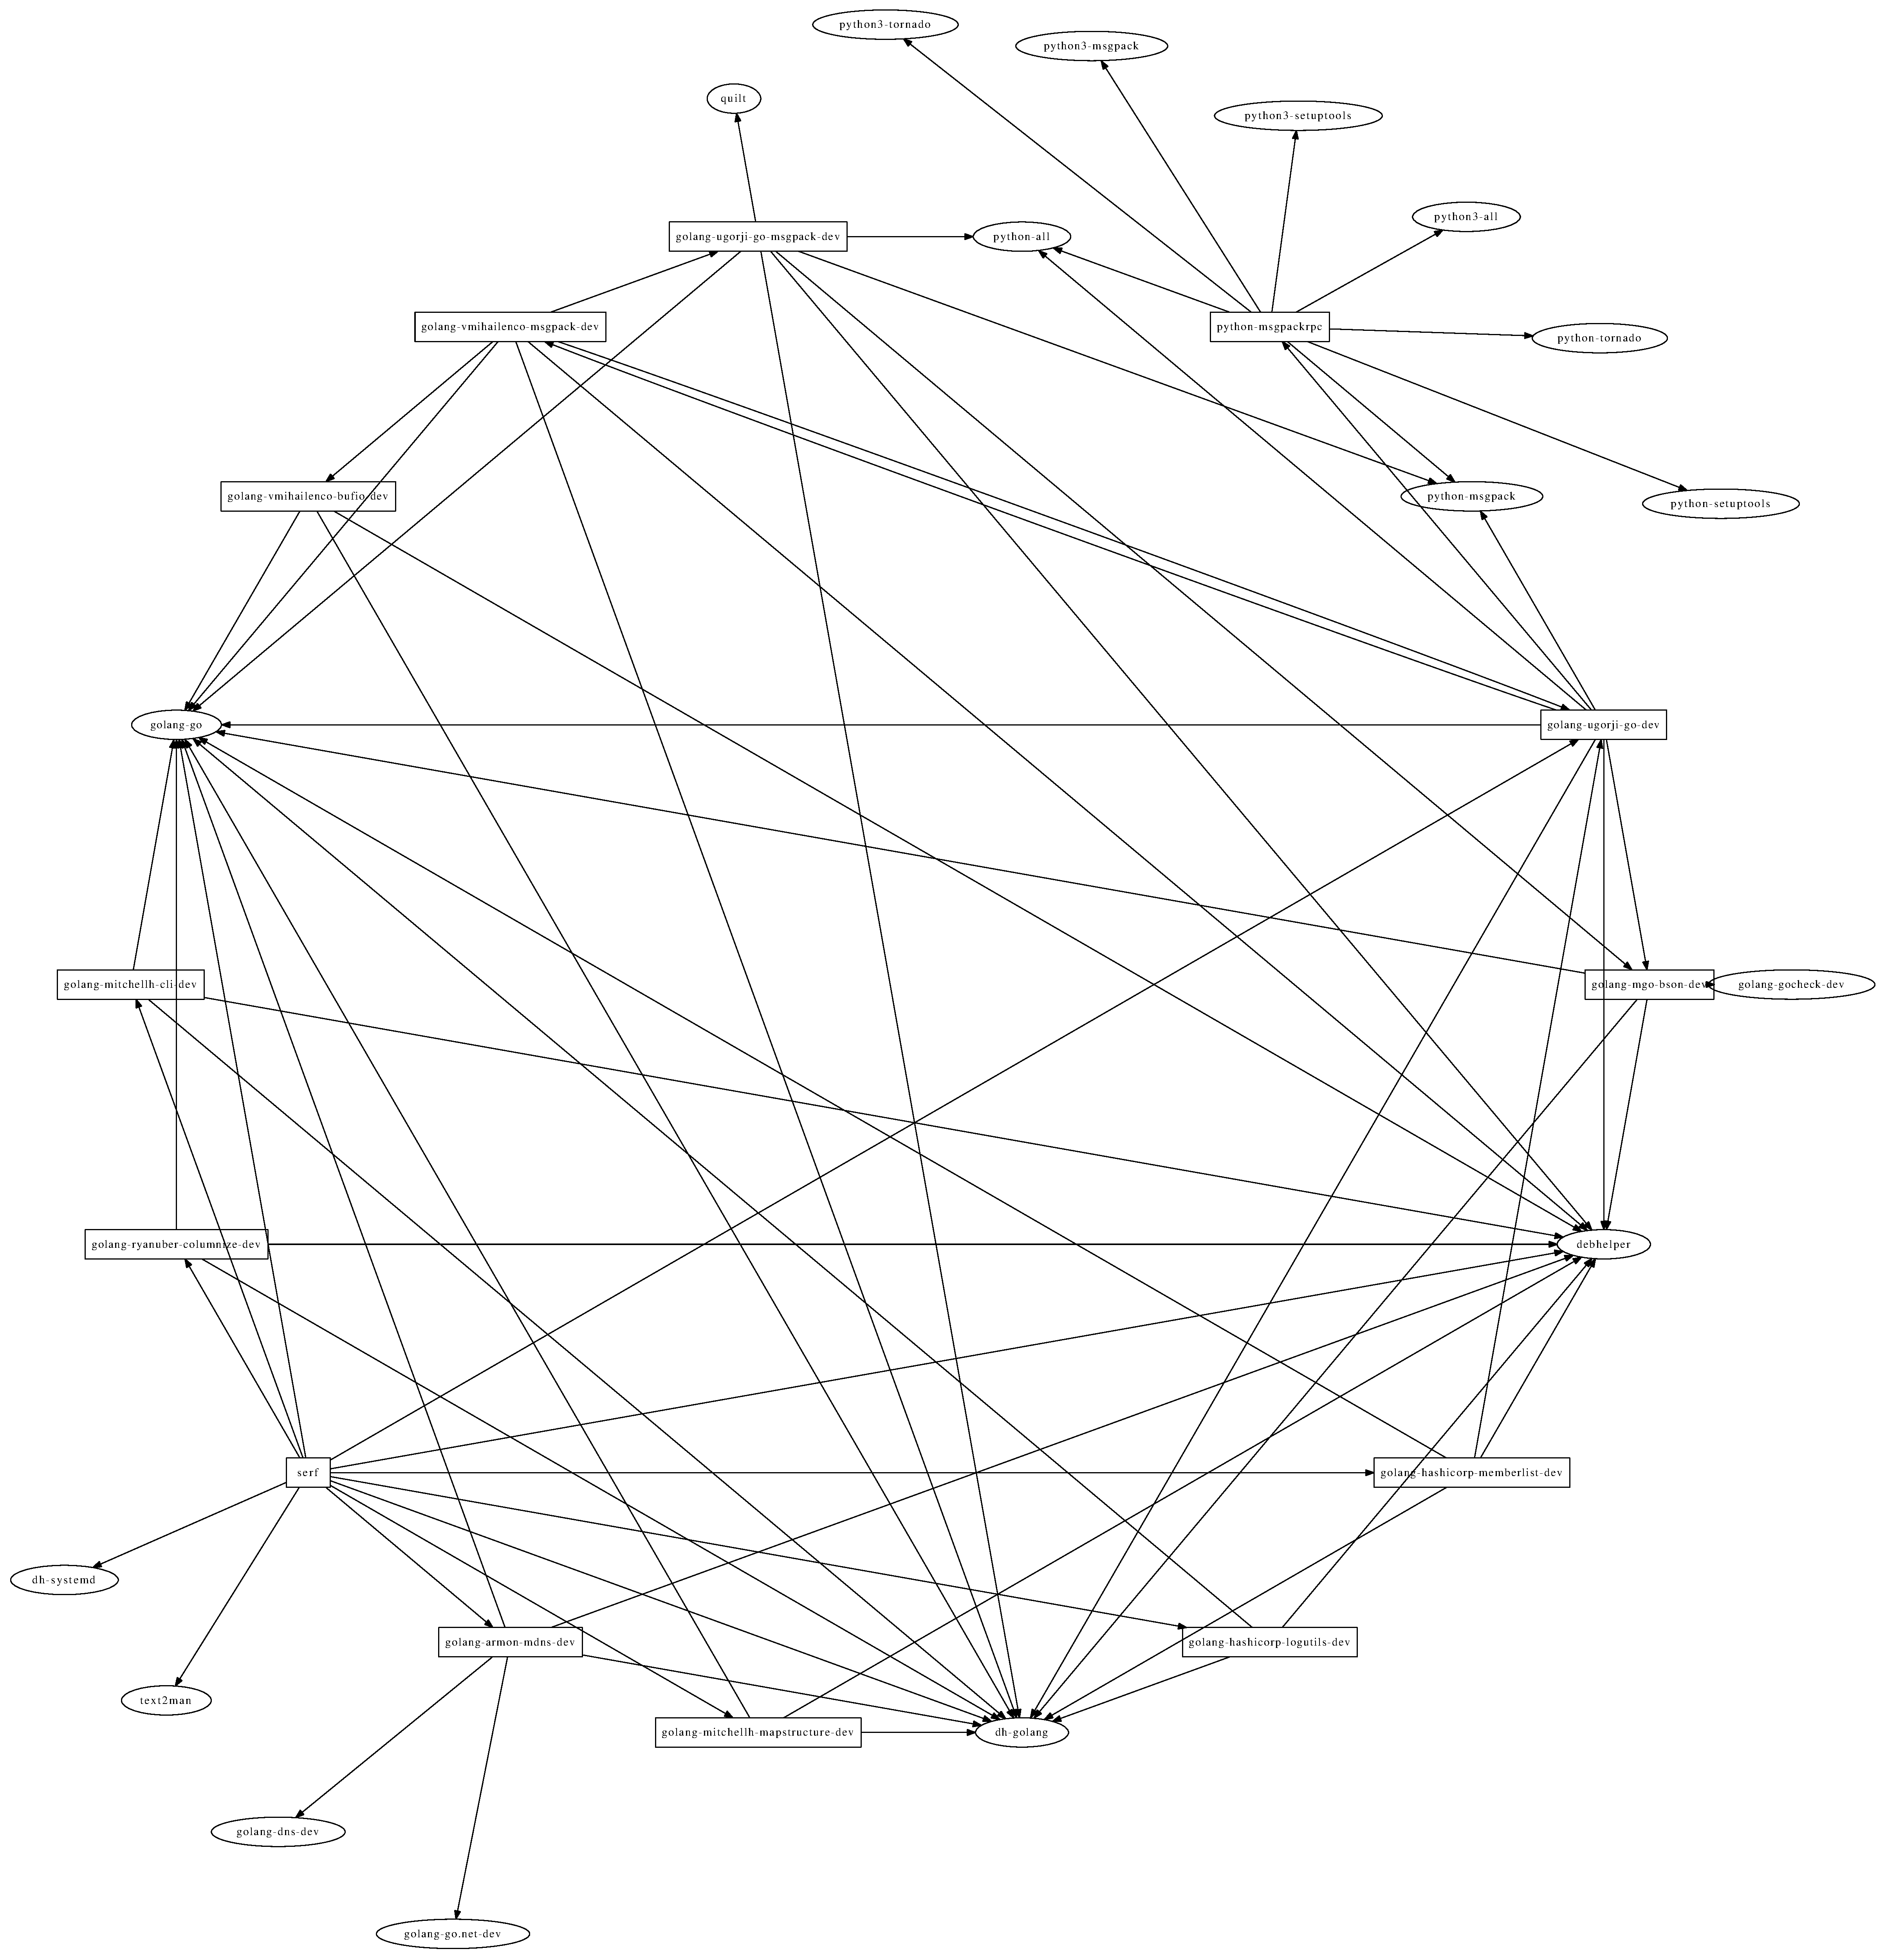
\includegraphics[width=15cm]{image201404/serf-dependency.eps}

\begin{thebibliography}{0}
  \bibitem{command-go}
    {\footnotesize{
        The Go Programming Language, ``Command go'',
        \url{http://golang.org/cmd/go/}}}
  \bibitem{debian-go-packaging}
    {\footnotesize{
        Alioth, ``Debian Go Packaging'',
        \url{http://pkg-go.alioth.debian.org/packaging.html}}}
\end{thebibliography}

%201401 kansai LTのためなし
%201402 kansai LTのためなし
%201402 tokyo OSC Tokyoのためなし
%201403 kansai LTのため無し
%201405 kansai もくもく会のみのため無し

%-------------------------------------------------------------------------------
\dancersection{Debian Trivia Quiz}{野島 貴英}
%-------------------------------------------------------------------------------

ところで、みなさん Debian 関連の話題においついていますか?Debian関連の話
題はメーリングリストをよんでいると追跡できます。ただよんでいるだけではは
りあいがないので、理解度のテストをします。特に一人だけでは意味がわからな
いところもあるかも知れません。みんなで一緒に読んでみましょう。

今回の出題範囲は\url{debian-devel-announce@lists.debian.org} や \url{debian-devel@lists.debian.org}に投稿された
内容とDebian Project Newsからです。

\begin{multicols}{2}
%; whizzy-master ../debianmeetingresume201311.tex
% $B0J>e$N@_Dj$r$7$F$$$k$?$a!"$3$N%U%!%$%k$G(B M-x whizzytex $B$9$k$H!"(Bwhizzytex$B$,MxMQ$G$-$^$9!#(B
%

\santaku
{2013/12/15$B$K=P$?(BDebian wheezy$B$N%"%C%W%G!<%H$N%P!<%8%g%s$O!)(B}
{7.3}
{7.2}
{7.1}
{A}
{debian wheezy$B$r$*;H$$$N3'MM$OAaB.%"%C%W%G!<%H$7$^$7$g$&!*(B}

\santaku
{Debian$B$b;22C$7$F$$$k(BFOSS$B9W8%<T$K=w@-$rA}$d$=$&1?F0$N;v$r$J$s$H$$$&!)(B}
{Encourage Women in Linux}
{Outreach Program For Women}
{IT$B@o;N(B}
{B}
{Outreach Program For Women($BN,$7$F(BOPW)$B$O!"(B\\
\url{http://gnome.org/opw/}
$B$K>pJs$,$"$j$^$9!#(B}

\santaku
{$B@hF|(BDebian$B$N(BTechnical Committee$B$K%a%s%P$,A}$($^$7$?!#$H$3$m$G!"(B
 $B8=:_$N(BTechnical Comittee$B$N(Bchair man$B$OC/$G$7$g$&(B?}
{Takahide Nojima}
{Lucas Nussbaum}
{Bdale Garbee}
{C}
{$B85(BHP$B$N(BLinux$BItLg$N(BCTO$B$rL3$a$?$H$$$&7PNr$N;}$A<g$G$9!#(Bdebconf$B$H$+$K(B
$B;22C(B/$B%S%G%*;kD0$H$+$9$k$H$o$+$k$N$G$9$,!">oO"$5$s$N$h$&$G$9!#(B}


%; whizzy-master ../debianmeetingresume201311.tex
% $B0J>e$N@_Dj$r$7$F$$$k$?$a!"$3$N%U%!%$%k$G(B M-x whizzytex $B$9$k$H!"(Bwhizzytex$B$,MxMQ$G$-$^$9!#(B
%

\santaku
{PHP$B$N%a%s%F%J%A!<%`$r#3$D$KJ,3d$9$k;v$,Ds0F$5$l$^$7$?!#J,3d$5$l$?%0%k!<%W$NL>A0$G4V0c$C$F$$$k$N$O$I$l!)(B}
{Debian PHP PECL Maintainers}
{Debian PHP PEAR Maintainers}
{Debian PHP DOCUMENT Maintainers}
{C}
{$B@5$7$/$O(B''Debian PHP Maintainers''$B$G$9!#0JA0!"(BDebian PHP Maintainers$B$O!"(BPHP$BK\BN$N%Q%C%1!<%8$b!"(BPEAR$B%b%8%e!<%k$N%Q%C%1!<%8$bN>J}%a%s%F%J%s%9$7$F$$$^$7$?!#(B}

\santaku
{Debian$B$K$D$$$F!"(BDebian Developer$B0J30$N?M$G$b9W8%$7$?$r;>$($^$7$g$&$H$$$&$3$H$G!":n$i$l$?%5%$%H$O!)(B}
{advocates.debian.org}
{contributors.debian.org}
{superstar.debian.org}
{B}
{Debian$B$K9W8%$7$?(BDebian Developer$B0J30$N?M$N%"%+%&%s%H$,(B\url{http://contributors.debian.org/}$B$K%j%9%H%"%C%W$5$l$k$h$&$K$J$j$^$7$?!#$J$*!"9W8%$K$D$$$F$N=87W$N85$O!"(B\url{https://contributors.debian.org/sources/}$B$K7G:\$5$l$F$$$k>pJs$r85$K=87W$7$F$$$k$H$N;v$G$9!#(B}

\santaku
{s390x$B%"!<%-%F%/%A%c$N%G%U%)%k%H(BC$B%3%s%Q%$%i$H$7$F$N(Bgcc$B$N%P!<%8%g%s$,JQ99$5$l$^$7$?!#$I$N%P!<%8%g%s$K$J$C$?$N$G$7$g$&!)(B}
{4.8}
{4.7}
{4.6}
{A}
{powerpc/ia64/sparc$B%"!<%-%F%/%A%c$N%G%U%)%k%H(BC$B%3%s%Q%$%i$O$^$@(Bgcc 4.6$B$N$h$&$G$9!#(BDebian$B$N<!4|%P!<%8%g%s$N(BJessie$B$G$O(Bgcc 4.6$B$O%5%]!<%HBP>]30$J$N$GAa$$$H$3$m(Bgcc 4.6$B$+$iC&5Q$9$kI,MW$,$"$j$^$9!#(B}

\santaku
{$B@hF|M-L>$J%G!<%?%Y!<%9$,%Q%C%1!<%8$H$7$FDI2C$5$l$^$7$?!#2?$H$$$&%G!<%?%Y!<%9$G$7$g$&$+!)(B}
{Maria DB}
{Percona DB}
{GDB}
{A}
{Maria DB$B$O!"(BLAMP$B%7%9%F%`$GM-L>$J(BMysql DB$B$NJL$N<BAu$G$9!#$D$$$K(BMaria DB$B%-%?!<!*:#8e$N(BMysql$B0MB8$N(BDebian$B$N%Q%C%1!<%8$NF08~$,5$$K$J$k$3$N:"$G$9!#(B}



%; whizzy-master ../debianmeetingresume201311.tex
% $B0J>e$N@_Dj$r$7$F$$$k$?$a!"$3$N%U%!%$%k$G(B M-x whizzytex $B$9$k$H!"(Bwhizzytex$B$,MxMQ$G$-$^$9!#(B
%

\santaku
{$B@hF|!"<!4|(BDebian$B$N%P!<%8%g%s$G$"$k(BJessie$B$K$F!"$H$"$k%"!<%-%F%/%A%c$N%5%]!<%H$,BG$A@Z$i$l$^$7$?!#$=$l$O!"$I$N%"!<%-%F%/%A%c!)(B}
{hurd-i386}
{s390x}
{ia64}
{C}
{$BD9$$4V$*Hh$l!*!d(Bia64$B!#(BAMD$B$N@oN,$KIi$1$?!"@$4V$KIi$1$?!#$H$3$m$G!"(Bhurd-i386$B%"!<%-%F%/%A%c$H(Bsparc$B%"!<%-%F%/%A%c$b!"(BRelease Team$B$K$h$l$P$o$j$H33$C$W$A$J>u67$N$h$&$G$9!#;29M!'(B\url{https://lists.debian.org/debian-devel-announce/2014/01/msg00008.html}}

\santaku
{$B:#7n(B2$B7n$"$?$^$K%j%j!<%9$5$l$?(Bstable$BHG$N(BDebian$B$N%P!<%8%g%s$O$$$/$D$G$7$g$&!)(B}
{7.3}
{7.4}
{7.5}
{B}
{wheezy$B;H$$$N?M$OAaB.%"%C%W%G!<%H$@!*:#2s$b%;%-%e%j%F%#$K4X$9$k(BBugfix$B$,<g$G$9!#(B}

\santaku
{Debian$B$N;q;:(B(Asset$B$N;v$G$9(B)$B$rG$$;$k$3$H$N$G$-$k!V?.Mj$KB-$kAH?%(B(Trusted Organization)$B!W$NDj5A$,@hF|%l%S%e!<$5$l$F$$$^$7$?!#?.Mj$KB-$kAH?%$N>r7o$KEv$F$O$^$i$J$$AH?%$O$I$l(B}
{$B8x<0(BDebian$B3+H/<T$,5o$J$$AH?%(B}
{$BAGAa$$1~Ez(B/$BBP1~$,$G$-$kAH?%(B}
{Debian$B<R2q7{>O$HBPN)$7$J$$AH?%(B}
{A}
{$B:G?7HG$O!"(B\url{https://wiki.debian.org/Teams/DPL/TrustedOrganizationCriteria}
$B$K7G:\$5$l$F$$$^$9!#$A$J$_$K!"?.Mj$KB-$kAH?%$,2?$r$9$k$N$+$NDj5A$K$D$$$F$O!"(BDebian$B%W%m%8%'%/%H7{>O$N(B9.4$B>O$K$"$j$^$9!#:#$^$GL@3N$J4p=`$,$J$+$C$?$N$+!)$H$$$&$N$,$A$g$C$H6C$-!#(B}

\santaku
{1/23$B$K(BPC$B%2!<%`$r%M%C%H$GGd$k%5!<%S%9(B(Steam)$B1?1D$GM-L>$J(BValve$B<R$,!"$$$/$D$+$N(BLinux$BBP1~$N%2!<%`$rL5NA$GDs6!$7$^$9$H7h$a$^$7$?!#$I$s$J?M$,BP>]$G$7$g$&$+!)(B}
{$BA4(BDebian$B%f!<%6(B}
{$BA4(BDebian$B8x<03+H/<T(B}
{$BA4(BIT$B4k6H$N(BDebian$B%5!<%P!<@o;N(B}
{B}
{$B$3$l$b%3%_%e%K%F%#$X$N4k6H$N4sIU$NJ}K!$H$7$FLLGr$$$H;W$$$^$7$?!#$$$o$f$k!V8=J*;Y5k!W$H$$$&E[$G$9$J!#(B}

\santaku
{Debian$B$N8xJs%A!<%`$,!"%=!<%7%c%k%a%G%#%"$N8x<0%"%+%&%s%H$G$NH/8@$9$kFbMF$NJg=8$r$7$F$$$^$9!#:G=i$KEj9F$5$l$k$N$O$I$N%"%+%&%s%H$G$7$g$&$+!)(B}
{twitter$B$N(Bdebian}
{google$B!\$N(Bdebian}
{identi.ca$B$N(Bdebian}
{C}
{debian$B$N%=!<%7%c%k%a%G%#%"$N8x<0%"%+%&%s%H$+$i(BDebian$B$N3hF0$r%"%T$j$?$$?M$O1~Jg$7$F$_$k$HNI$$$H$*$b$$$^$9!#(B\url{https://wiki.debian.org/Teams/Publicity/Identica}}

\santaku
{Debian Member$B$X(BSIP$B%5!<%S%9$,Ds6!$5$l$^$7$?!#(BDebian Member$B$8$c$J$$?M$,(BDebian Member$B$H(BSIP$B$r;H$C$?%3%_%e%K%1!<%7%g%s$r$9$k$H$-$KJXMx$J%5%$%H$O!)(B}
{rtc.debian.org}
{freephonebox.net}
{www.nttdocomo.co.jp}
{B}
{DSA$B4hD%$C$?(B!Debian Member$B$N?M$O(B\url{rtc.debian.org}$B$K(Bxxxx$B!w(Bdebian.org$B$r(BSIP$B%"%+%&%s%H$K$7$F%m%0%$%s$7$F$*$/$H!"(BDebian Member$B0J30$N?M$O(Bfreephonebox.net$B$+$i(Bxxxx$B!w(Bdebian.org$B08$KO"Mm$r<h$k$3$H$,$G$-$k$H$N;v!#(B}

\santaku
{Debconf14$B$N3+:EF|$O!)(B}
{8$B7n(B23$BF|!A(B31$BF|(B}
{8$B7n(B10$BF|!A(B24$BF|(B}
{7$B7n(B21$BF|!A(B31$BF|(B}
{A}
{$B:#G/$O%"%a%j%+!!%*%l%4%s=#!!%]!<%H%i%s%I$G3+$+$l$^$9!#@hF|%9%]%s%5!<Jg=8$N0FFb$,N.$l$^$7$?!#(BDebconf14$B$K$D$$$F$O(B\url{http://debconf14.debconf.org/}$B!#(BDebconf13$B$NMM;R$O(B\url{http://www.irill.org/videos/debconf13}$B$G8+$l$^$9!#(B}

\santaku
{Jessie$B$N%G%U%)%k%H$N(Binit$B%7%9%F%`$,EjI<$K$h$j7hDj$7$^$7$?!#$5$F2?$K$J$C$?$G$7$g$&!)(B}
{sysvinit}
{upstart}
{systemd}
{C}
{$BD9$$4V$NO@Ah$K%1%j$,$D$$$?$h$&$G$9!#AaB.(Bsystemd$B$N;H$$J}$r3P$($J$$$H!#(B
 $B;29M(B:ctte$B$NEjI<%"%J%&%s%9(B\url{https://lists.debian.org/debian-ctte/2014/02/msg00281.html}$B!"7kO@(B\url{https://lists.debian.org/debian-ctte/2014/02/msg00405.html}
}

%; whizzy-master ../debianmeetingresume201311.tex
% 以上の設定をしているため、このファイルで M-x whizzytex すると、whizzytexが利用できます。
%

\santaku
{2014年GSoCのメンター募集が行われています。2014年のGSoCにて採択されていないものはどれ}
{hurd-i386の開発}
{clangでDebianのパッケージをコンパイルできるようにする}
{Android上でDebian環境を作れる件の改良を行う}
{A}
{他にもいろいろなProjectがDebian Projectから採択されています。Elektra\url{http://www.libelektra.org}で設定ファイルのアップグレードを改良するとか、libstdc++からlibc++を使うようにDebianを変更する件や、パッケージ管理にMuonを使う件など。参考:\url{https://wiki.debian.org/SummerOfCode2014/Projects}}

\santaku
{2014/2/14にバグレポートのIDが\#740000を向かえました。\#730000からどのぐらいの期間がたったでしょう?}
{1ヶ月と3日}
{3ヶ月と4日}
{10ヶ月と10日}
{B}
{毎年、Christian Perrierさんにより、バグレポートのIDについて、将来いつ何万番台を迎えるかについて当てるコンテストが行われています。}

\santaku
{Debianのコミュニティにより提供されているWebサービスについて調査が行われています。この調査の名前は?}
{Debian Services Servey}
{Outreach Program For Women}
{Debian Services Census}
{C}
{2014/2/13に呼びかけが行われました。現在のサービスの名前とURLのリストは、\url{https://wiki.debian.org/Services}にまとめられています。}

\santaku
{毎年恒例のDPL選挙が始まりました。2014年のDPL立候補者は誰?}
{Takahide Nojima}
{Lucas Nussbaum}
{Stefano Zacchiroli}
{B}
{lucusは2013年DPLですが、2年連続立候補となります。他の2名の方は、Gergely Nagyさん、Neil McGovernさんとなります。
 選挙期間は2014/3/31〜4/13となります。各候補者の声明は、\url{http://www.debian.org/vote/2014/platforms/}に掲載予定です。}

%; whizzy-master ../debianmeetingresume201311.tex
% $B0J>e$N@_Dj$r$7$F$$$k$?$a!"$3$N%U%!%$%k$G(B M-x whizzytex $B$9$k$H!"(Bwhizzytex$B$,MxMQ$G$-$^$9!#(B
%

\santaku
{2015$BG/$N(BDebconf15$B$N3+:E9q$O$I$3$K$J$C$?$G$7$g$&!)(B}
{$B%\%9%K%"!&%X%k%D%'%4%S%J(B}
{$B%&%/%i%$%J(B}
{$B%I%$%D(B}
{C}
{$B:#EY$O%I%$%D$@$=$&$G$9!#$A$J$_$K:#G/$N(BDebconf14$B$O(B8/23-31$B$G(BUSA$B$N(BPortland,Oregon
$B$G3+:EM=Dj$G$9!#(B}

\santaku
{DPL$BA*5s$,9T$o$l$^$7$?!#:#G/$N(BDPL$B$OC/$K$J$C$?$G$7$g$&$+!)(B}
{Lucas Nussbaum}
{Neil McGovern}
{Rapha\"{e}l Hertzog}
{A}
{$B:#G/$N(BDPL$B$N8uJd<T$O#2L>$G!"(BLucas Nussbaum$B$5$s!"(BNeil McGovern$B$5$s$N#2L>(B
$B$G$7$?!##2L>$H$b<+A&$H$N$3$H$G$9!#A*5s$N7k2L!"(B
Lucas Nussbaum(lucus)$B$5$s$N05>!$@$C$?$h$&$G$9!#$A$J$_$K!"(B
Rapha\"{e}l Hertzog$B$5$s$O!"(BThe Debian 
Administrator\'s handbook$B$N:n<T!"B>$K$b0N6H$,$?$/$5$s!#(B}

\santaku
{clang3.4$B$K$h$k(BDebian$B%Q%C%1!<%8$N:F9=C[$,9T$o$l$^$7$?!#7k2L2?(B\%$B$N%Q%C%1!<%8$,@.8y$7$?$G$7$g$&$+!)(B}
{90\%}
{50\%}
{10\%}
{A}
{\url{http://clang.debian.net/}$B$,(Bclang$B$K$h$k(BDebian$B%Q%C%1!<%8:F9=C[$N%]!<%?%k%5%$%H$G$9!#KhG/!"(Bclang$B$N%P!<%8%g%s$r>e$2$F!"A4(BDebian$B%Q%C%1!<%8$r:F9=C[$7$?7k2L$,:\$j$^$9!#:#G/$N7k2L$H$7$F$O:F9=C[BP>]$N%Q%C%1!<%8$N?t$,5nG/$HBgI}$KA}$($F$$$k$K$b$+$+$o$i$:!"9=C[<:GT$K=*$o$C$?%Q%1!<%8?t$,5nG/$HJQ$o$i$J$+$C$?$H$$$&Hs>o$KNI$$7k2L$H$J$C$F$$$^$9!#(B}

\santaku
{beagle board$B%7%j!<%:$H$$$&Hs>o$K?M5$$N$"$k(BARM$B$N<B83%\!<%I$K%P%s%I%k$5$l$k(BOS$B$N>-Mh$N8+DL$7$K$D$$$F!"(Bbeagle board$B$NAON)<T$,$I$N(BOS$B$K$9$kM=Dj$HH/8@$7$?$+!)(B}
{Gentoo}
{Debian$B$C$7$g!*(BDebian}
{Andoroid OS}
{B}
{\url{http://opensource.com/life/14/3/interview-jason-kridner-beagleboard}
$B$K$F!">-Mh(BDebian$B$K$9$k$H$$$&H/8@$,$"$j$^$9!#$H$3$m$G!"(Bbeagle board$B%7%j!<%:$OL$$@$K(BOMAP$B$r(B
$B;H$$B3$1$k$N$+$,6=L#DE!9$G$O$"$j$^$9!#(B}

\santaku
{$B7cO@$NKv!"(B3$B7nCf=\:"$K(BDebian$B$N(Bca-certificates$B%Q%C%1!<%8$+$i>C$($?(Broot$B>ZL@=q$,$"$j$^$9!#$=$l$O$J$s$G$7$g$&!)(B}
{RapidSSL$B$N(Broot$B>ZL@=q(B}
{CAcert$B$N(Broot$B>ZL@=q(B}
{Verisign$B$N(Broot$B>ZL@=q(B}
{B}
{$B5DO@$N%5%^%j$O!"(BLWN$B$N5-;v(B\url{https://lwn.net/Articles/590879/}$B$,H=$j$d$9$$$G$9!#$^$?!"(BCAcert$B$C$F2?!)$H$$$&J}$O!"Bh(B71$B2sEl5~%(%j%"(BDebian$BJY6/2q(B(2010$BG/(B12$B7n3+:E(B)\url{http://tokyodebian.alioth.debian.org/2010-12.html}$B$K7G:\$5$l$F$$$kJY6/2q;qNA$,$*4+$a$G$9!#(B}

\santaku
{Jessie$B$K$F%G%9%/%H%C%W4D6-$rA*Br$7$?:]$KF3F~$5$l$k!"%G%U%)%k%H%3%_%e%K%1!<%7%g%s%D!<%k$N8uJd$K$D$$$F5DO@$,$5$l$F$$$j$^$9!#0J2<$N$I$l$G$7$g$&!)(B}
{Empathy}
{licq}
{jitsi}
{C}
{Debian$B$G$O!"%G%U%)%k%H$N%3%_%e%K%1!<%7%g%s%D!<%k$H$7$F!"$[$\40A4$K(BRTC/VoIP$B$r%5%]!<%H$9$k$3$H$,K>$^$7$$$H$5$l$?$?$a!"$3$A$i$K8~$$$F$$$k%D!<%k$H$7$F:#$^$G$N(BEmpathy$B$h$j$b(Bjitsi$B$,8~$$$F$$$k$N$G$O!)$H$$$&$3$H$+$i5DO@$,3+;O$5$l$^$7$?!#(B}

\santaku
{$B@hF|(BDebian$B$K(BOTR$B%A!<%`$H$$$&(BOTR$B%=%U%H$r%Q%C%1!<%82=$9$k%0%k!<%W$,7k@.$5$l$^$7$?!#$H$3$m$G(BOTR$B$C$F$J$s$NN,!)(B}
{Owa-Tte-Ru}
{OpticalTRacking}
{Off-the-Record}
{C}
{Off-the-Record$B$H$O!"0E9f2=5;=Q$r;H$C$F%$%s%U%iDs6!<T$K$9$i%a%C%;!<%8$N$d$j$H$j$NFbMF$r8+$;$J$$!J5-O?$5$;$J$$!K%a%C%;!<%8%5!<%S%9$rL\;X$7$?$b$N$G$9(B\url{https://www.otr.im/}$B!#(B}

\santaku
{$B@hF|!"(BDebian squeeze$B$N%5%]!<%H4|4V$,?-$S$k@k8@$,(BDSA$B$K$h$j%"%J%&%s%9$5$l$^$7$?!#7k6I$$$D$K$J$C$?!)(B}
{2015/2}
{2016/2}
{2016/5}
{B}
{Long Term Support(LTS)$B$@$=$&$G$9(B\url{https://lists.debian.org/debian-security-announce/2014/msg00082.html}$B!#M=Dj$G$O!"(B2014/5/31$B:"$K%5%]!<%H=*N;$9$k$O$:$G$7$?$N$G!"#2G/<e$N1dD9$H$J$j$^$9!#$?$@%5%]!<%H1dD9$5$l$k$N$O!"(BDebian squeeze$B$NA4It$N%Q%C%1!<%8$G$O$J$$$N$G!"%5%]!<%H$5$l$J$$%Q%C%1!<%8$r==J,$K$*;H$$$N3'MM$O!"(BDebian wheezy$B$X%"%C%W%0%l!<%I$9$k$3$H$r$*4+$a$7$F$*$-$^$9!#(B}



%; whizzy-master ../debianmeetingresume201311.tex
% 以上の設定をしているため、このファイルで M-x whizzytex すると、whizzytexが利用できます。
%

\santaku
{2014/4/26に、とあるアーキテクチャがtestingから外されました。次のうちのどれでしょう?}
{i386}
{armel}
{sparc}
{C}
{リリースチームの見解によれば、ツールチェインの問題、安定性の問題、また今後Jessieリリースに向けての開発について明確な見解が開発チームらから得られなかったとのことです。}

\santaku
{2014/4/26にdebianの安定版がリリースされました。バージョンはいくつでしょう?}
{7.4}
{7.5}
{7.6}
{B}
{5回目の更新リリースとなります。安定版を使っている人でアップデートしていない人は、早速apt-get upgradeをお勧めしておきます。主にバグフィックスとセキュリテイ対策となります。}




\end{multicols}

% 索引
\printindex

% 問題と回答が同じみひらきにならないようにする
%\cleartoevenpage
%-------------------------------------------------------------------------------
\dancersection{Debian Trivia Quiz 問題回答}{野島 貴英}
%-------------------------------------------------------------------------------
\\
{\small
 Debian Trivia Quiz の問題回答です。 あなたは何問わかりましたか? \\
 %回答はdebianmeetingresume2013-fuyu.jqzというファイルに生成されるので、
 %それを手動でコピペして使う。
 % ここからコピペ
 % FIXME 問題が全部はいったらコピペすること
 %(progn (next-line 1)(insert-file "debianmeetingresume2013-fuyu.jqz") )
1. A debian wheezyをお使いの皆様は早速アップデートしましょう!\\
2. B Outreach Program For Women(略してOPW)は、\\ \url {http://gnome.org/opw/} に情報があります。\\
3. C 元HPのLinux部門のCTOを務めたという経歴の持ち主です。debconfとかに参加/ビデオ視聴とかするとわかるのですが、常連さんのようです。\\
4. C 正しくは''Debian PHP Maintainers''です。以前、Debian PHP Maintainersは、PHP本体のパッケージも、PEARモジュールのパッケージも両方メンテナンスしていました。\\
5. B Debianに貢献したDebian Developer以外の人のアカウントが\url {http://contributors.debian.org/}にリストアップされるようになりました。なお、貢献についての集計の元は、\url {https://contributors.debian.org/sources/}に掲載されている情報を元に集計しているとの事です。\\
6. A 2013/12/23現在、powerpc/ia64/sparcアーキテクチャのデフォルトCコンパイラはまだgcc 4.6のようです。Debianの次期バージョンのJessieではgcc 4.6はサポート対象外なので早いところgcc 4.6から脱却する必要があります。\\
7. A Maria DBは、LAMPシステムで有名なMysql DBの別の実装です。ついにMaria DBキター!今後のMysql依存のDebianのパッケージの動向が気になるこの頃です。\\
8. C 長い間お疲れ!>ia64。AMDの戦略に負けた、世間に負けた。ところで、hurd-i386アーキテクチャとsparcアーキテクチャも、2014/1時点でRelease Teamによればわりと崖っぷちな状況のようです。 参考:\url{https://lists.debian.org/debian-devel-announce/2014/01/msg00008.html} \\
9. B wheezy使いの人は早速アップデートだ!今回もセキュリティに関するBugfixが主です。\\
10. A 最新版は、\url {https://wiki.debian.org/Teams/DPL/TrustedOrganizationCriteria} に掲載されています。ちなみに、信頼に足る組織が何をするのかの定義については、Debianプロジェクト憲章の9.4章にあります。今まで明確な基準がなかったのか?というのがちょっと驚き。\\
11. B これもコミュニティへの企業の寄付の方法として面白いと思いました。いわゆる「現物支給」という奴ですな。\\
12. C debianのソーシャルメディアの公式アカウントからDebianの活動をアピりたい人は応募してみると良いとおもいます。\url {https://wiki.debian.org/Teams/Publicity/Identica}\\
13. B DSA頑張った!Debian Memberの人は\url {rtc.debian.org}にxxxx@debian.orgをSIPアカウントにしてログインしておくと、Debian Member以外の人はfreephonebox.netからxxxx@debian.org宛に連絡を取ることができるとの事。\\
14. A 2014年はアメリカ オレゴン州 ポートランドで開かれます。先日スポンサー募集の案内が流れました。Debconf14については\url {http://debconf14.debconf.org/}。Debconf13の様子は\url {http://www.irill.org/videos/debconf13}で見れます。\\
15. C 長い間の論争にケリがついたようです。早速systemdの使い方を覚えないと。参考:ctteの投票アナウンス\url {https://lists.debian.org/debian-ctte/2014/02/msg00281.html}、結論\url {https://lists.debian.org/debian-ctte/2014/02/msg00405.html} \\
16. A 他にもいろいろなProjectがDebian Projectから採択されています。Elektra\url {http://www.libelektra.org}で設定ファイルのアップグレードを改良するとか、libstdc++からlibc++を使うようにDebianを変更する件や、パッケージ管理にMuonを使う件など。参考:\url {https://wiki.debian.org/SummerOfCode2014/Projects}\\
17. B 毎年、Christian Perrierさんにより、バグレポートのIDについて、将来いつ何万番台を迎えるかについて当てるコンテストが行われています。\\
18. C 2014/2/13に呼びかけが行われました。現在のサービスの名前とURLのリストは、\url{https://wiki.debian.org/Services}にまとめられています。\\
19. B lucusは2013年DPLですが、2年連続立候補となります。他の2名の方は、Gergely Nagyさん、Neil McGovernさんとなります。 選挙期間は2014/3/31〜4/13となります。各候補者の声明は、\url{http://www.debian.org/vote/2014/platforms/}に掲載予定です。\\
20. C 2015年はドイツだそうです。ちなみに2014年のDebconf14は8/23-31でUSAのPortland,Oregon で開催予定です。 \\
21. A 2014年のDPLの候補者は2名で、Lucas Nussbaumさん、Neil McGovernさんの2名でした。2名とも自薦とのことです。選挙の結果、Lucas Nussbaum(lucus)さんの圧勝だったようです。ちなみに、Rapha\"{e}l Hertzogさんは、The Debian Administrator\'s handbookの作者、他にも偉業がたくさん。\\
22. A \url {http://clang.debian.net/}がclangによるDebianパッケージ再構築のポータルサイトです。毎年、clangのバージョンを上げて、全Debianパッケージを再構築した結果が載ります。2014/1の結果としては再構築対象のパッケージの数が2013/1より大幅に増えているにもかかわらず、構築失敗に終わったパケージ数が変わらなかったという非常に良い結果となっています。\\
23. B \url {http://opensource.com/life/14/3/interview-jason-kridner-beagleboard} にて、将来Debianにするという発言があります。ところで、beagle boardシリーズは未だにOMAPを使い続けるのかが興味津々ではあります。\\
24. B 議論のサマリは、LWNの記事\url {https://lwn.net/Articles/590879/}が判りやすいです。また、CAcertって何?という方は、第71回東京エリアDebian勉強会(2010年12月開催)\url {http://tokyodebian.alioth.debian.org/2010-12.html}に掲載されている勉強会資料がお勧めです。\\
25. C Debianでは、デフォルトのコミュニケーションツールとして、ほぼ完全にRTC/VoIPをサポートすることが望ましいとされたため、こちらに向いているツールとして今までのEmpathyよりもjitsiが向いているのでは?ということから議論が開始されました。\\
26. C Off-the-Recordとは、暗号化技術を使ってインフラ提供者にすらメッセージのやりとりの内容を見せない(記録させない)メッセージサービスを目指したものです\url {https://www.otr.im/}。\\
27. B Long Term Support(LTS)だそうです\url {https://lists.debian.org/debian-security-announce/2014/msg00082.html}。予定では、2014/5/31頃にサポート終了するはずでしたので、2年弱の延長となります。ただサポート延長されるのは、Debian squeezeの全部のパッケージではないので、サポートされないパッケージを十分にお使いの皆様は、Debian wheezyへアップグレードすることをお勧めしておきます。\\
28. C リリースチームの見解によれば、ツールチェインの問題、安定性の問題、また今後Jessieリリースに向けての開発について明確な見解が開発チームらから得られなかったとのことです。 \\
29. B 5回目の更新リリースとなります。安定版を使っている人でアップデートしていない人は、早速apt-get upgradeをお勧めしておきます。主にバグフィックスとセキュリテイ対策となります。\\
}

\pagestyle{empty}
\cleartoevenpage

\newpage
{
\large
\begin{itembox}{\bf 『あんどきゅめんてっど でびあん』について}
本書は、東京および関西周辺で毎月行なわれている『東京エリア Debian 勉強会』(第107回から第113回)および
『関西 Debian 勉強会』(第83回)で
使用された資料・小ネタ・必殺技などを一冊にまとめたものです。
第80回から第82回、第84回、関西Debian勉強会はもくもく会のため無し、
第110回東京エリアDebian勉強会資料はオープンソースカンファレンス2014 Tokyo/Springのため無し、
% FIXME: 回数を修正すること。
内容は無保証、つっこみなどがあれば勉強会にて。
\end{itembox}
}

\vspace*{13cm}
{\color{dancerlightblue}\rule{\hsize}{1mm}}
\vspace{2mm}
\includegraphics[width=2cm]{image200502/openlogo-nd.eps}
\noindent \Large \bf あんどきゅめんてっど でびあん 2014年夏号\\
\noindent \normalfont 2014年8月12日 \hspace{5mm}  初版第1刷発行\\
\noindent \normalfont 東京エリア Debian 勉強会/関西エリア Debian 勉強会 (編集・印刷・発行)\\
{\color{dancerdarkblue}\rule{\hsize}{1mm}}

\end{document}
